
%% bare_jrnl.tex
%% V1.4b
%% 2015/08/26
%% by Michael Shell
%% see http://www.michaelshell.org/
%% for current contact information.
%%
%% This is a skeleton file demonstrating the use of IEEEtran.cls
%% (requires IEEEtran.cls version 1.8b or later) with an IEEE
%% journal paper.
%%
%% Support sites:
%% http://www.michaelshell.org/tex/ieeetran/
%% http://www.ctan.org/pkg/ieeetran
%% and
%% http://www.ieee.org/

%%*************************************************************************
%% Legal Notice:
%% This code is offered as-is without any warranty either expressed or
%% implied; without even the implied warranty of MERCHANTABILITY or
%% FITNESS FOR A PARTICULAR PURPOSE! 
%% User assumes all risk.
%% In no event shall the IEEE or any contributor to this code be liable for
%% any damages or losses, including, but not limited to, incidental,
%% consequential, or any other damages, resulting from the use or misuse
%% of any information contained here.
%%
%% All comments are the opinions of their respective authors and are not
%% necessarily endorsed by the IEEE.
%%
%% This work is distributed under the LaTeX Project Public License (LPPL)
%% ( http://www.latex-project.org/ ) version 1.3, and may be freely used,
%% distributed and modified. A copy of the LPPL, version 1.3, is included
%% in the base LaTeX documentation of all distributions of LaTeX released
%% 2003/12/01 or later.
%% Retain all contribution notices and credits.
%% ** Modified files should be clearly indicated as such, including  **
%% ** renaming them and changing author support contact information. **
%%*************************************************************************


% *** Authors should verify (and, if needed, correct) their LaTeX system  ***
% *** with the testflow diagnostic prior to trusting their LaTeX platform ***
% *** with production work. The IEEE's font choices and paper sizes can   ***
% *** trigger bugs that do not appear when using other class files.       ***                          ***
% The testflow support page is at:
% http://www.michaelshell.org/tex/testflow/



\documentclass[journal]{IEEEtran}
%
% If IEEEtran.cls has not been installed into the LaTeX system files,
% manually specify the path to it like:
% \documentclass[journal]{../sty/IEEEtran}





% Some very useful LaTeX packages include:
% (uncomment the ones you want to load)


% *** MISC UTILITY PACKAGES ***
%
%\usepackage{ifpdf}
% Heiko Oberdiek's ifpdf.sty is very useful if you need conditional
% compilation based on whether the output is pdf or dvi.
% usage:
% \ifpdf
%   % pdf code
% \else
%   % dvi code
% \fi
% The latest version of ifpdf.sty can be obtained from:
% http://www.ctan.org/pkg/ifpdf
% Also, note that IEEEtran.cls V1.7 and later provides a builtin
% \ifCLASSINFOpdf conditional that works the same way.
% When switching from latex to pdflatex and vice-versa, the compiler may
% have to be run twice to clear warning/error messages.






% *** CITATION PACKAGES ***
%
%\usepackage{cite}
% cite.sty was written by Donald Arseneau
% V1.6 and later of IEEEtran pre-defines the format of the cite.sty package
% \cite{} output to follow that of the IEEE. Loading the cite package will
% result in citation numbers being automatically sorted and properly
% "compressed/ranged". e.g., [1], [9], [2], [7], [5], [6] without using
% cite.sty will become [1], [2], [5]--[7], [9] using cite.sty. cite.sty's
% \cite will automatically add leading space, if needed. Use cite.sty's
% noadjust option (cite.sty V3.8 and later) if you want to turn this off
% such as if a citation ever needs to be enclosed in parenthesis.
% cite.sty is already installed on most LaTeX systems. Be sure and use
% version 5.0 (2009-03-20) and later if using hyperref.sty.
% The latest version can be obtained at:
% http://www.ctan.org/pkg/cite
% The documentation is contained in the cite.sty file itself.






% *** GRAPHICS RELATED PACKAGES ***
%
\ifCLASSINFOpdf
 \usepackage[pdftex]{graphicx}
  % declare the path(s) where your graphic files are
  % \graphicspath{{../pdf/}{../jpeg/}}
  % and their extensions so you won't have to specify these with
  % every instance of \includegraphics
  % \DeclareGraphicsExtensions{.pdf,.jpeg,.png}
\else
  % or other class option (dvipsone, dvipdf, if not using dvips). graphicx
  % will default to the driver specified in the system graphics.cfg if no
  % driver is specified.
  % \usepackage[dvips]{graphicx}
  % declare the path(s) where your graphic files are
  % \graphicspath{{../eps/}}
  % and their extensions so you won't have to specify these with
  % every instance of \includegraphics
  % \DeclareGraphicsExtensions{.eps}
\fi
% graphicx was written by David Carlisle and Sebastian Rahtz. It is
% required if you want graphics, photos, etc. graphicx.sty is already
% installed on most LaTeX systems. The latest version and documentation
% can be obtained at: 
% http://www.ctan.org/pkg/graphicx
% Another good source of documentation is "Using Imported Graphics in
% LaTeX2e" by Keith Reckdahl which can be found at:
% http://www.ctan.org/pkg/epslatex
%
% latex, and pdflatex in dvi mode, support graphics in encapsulated
% postscript (.eps) format. pdflatex in pdf mode supports graphics
% in .pdf, .jpeg, .png and .mps (metapost) formats. Users should ensure
% that all non-photo figures use a vector format (.eps, .pdf, .mps) and
% not a bitmapped formats (.jpeg, .png). The IEEE frowns on bitmapped formats
% which can result in "jaggedy"/blurry rendering of lines and letters as
% well as large increases in file sizes.
%
% You can find documentation about the pdfTeX application at:
% http://www.tug.org/applications/pdftex





% *** MATH PACKAGES ***
%
\usepackage{amsmath}
% A popular package from the American Mathematical Society that provides
% many useful and powerful commands for dealing with mathematics.
%
% Note that the amsmath package sets \interdisplaylinepenalty to 10000
% thus preventing page breaks from occurring within multiline equations. Use:
%\interdisplaylinepenalty=2500
% after loading amsmath to restore such page breaks as IEEEtran.cls normally
% does. amsmath.sty is already installed on most LaTeX systems. The latest
% version and documentation can be obtained at:
% http://www.ctan.org/pkg/amsmath
%\usepackage{amsaddr}		
%\usepackage{amsthm}		
%\usepackage{amsaddr}		
\usepackage{amsfonts}		





% *** SPECIALIZED LIST PACKAGES ***
%
%\usepackage{algorithmic}
% algorithmic.sty was written by Peter Williams and Rogerio Brito.
% This package provides an algorithmic environment fo describing algorithms.
% You can use the algorithmic environment in-text or within a figure
% environment to provide for a floating algorithm. Do NOT use the algorithm
% floating environment provided by algorithm.sty (by the same authors) or
% algorithm2e.sty (by Christophe Fiorio) as the IEEE does not use dedicated
% algorithm float types and packages that provide these will not provide
% correct IEEE style captions. The latest version and documentation of
% algorithmic.sty can be obtained at:
% http://www.ctan.org/pkg/algorithms
% Also of interest may be the (relatively newer and more customizable)
% algorithmicx.sty package by Szasz Janos:
% http://www.ctan.org/pkg/algorithmicx




% *** ALIGNMENT PACKAGES ***
%
%\usepackage{array}
% Frank Mittelbach's and David Carlisle's array.sty patches and improves
% the standard LaTeX2e array and tabular environments to provide better
% appearance and additional user controls. As the default LaTeX2e table
% generation code is lacking to the point of almost being broken with
% respect to the quality of the end results, all users are strongly
% advised to use an enhanced (at the very least that provided by array.sty)
% set of table tools. array.sty is already installed on most systems. The
% latest version and documentation can be obtained at:
% http://www.ctan.org/pkg/array


% IEEEtran contains the IEEEeqnarray family of commands that can be used to
% generate multiline equations as well as matrices, tables, etc., of high
% quality.




% *** SUBFIGURE PACKAGES ***
%\ifCLASSOPTIONcompsoc
%  \usepackage[caption=false,font=normalsize,labelfont=sf,textfont=sf]{subfig}
%\else
%  \usepackage[caption=false,font=footnotesize]{subfig}
%\fi
% subfig.sty, written by Steven Douglas Cochran, is the modern replacement
% for subfigure.sty, the latter of which is no longer maintained and is
% incompatible with some LaTeX packages including fixltx2e. However,
% subfig.sty requires and automatically loads Axel Sommerfeldt's caption.sty
% which will override IEEEtran.cls' handling of captions and this will result
% in non-IEEE style figure/table captions. To prevent this problem, be sure
% and invoke subfig.sty's "caption=false" package option (available since
% subfig.sty version 1.3, 2005/06/28) as this is will preserve IEEEtran.cls
% handling of captions.
% Note that the Computer Society format requires a larger sans serif font
% than the serif footnote size font used in traditional IEEE formatting
% and thus the need to invoke different subfig.sty package options depending
% on whether compsoc mode has been enabled.
%
% The latest version and documentation of subfig.sty can be obtained at:
% http://www.ctan.org/pkg/subfig




% *** FLOAT PACKAGES ***
%
%\usepackage{fixltx2e}
% fixltx2e, the successor to the earlier fix2col.sty, was written by
% Frank Mittelbach and David Carlisle. This package corrects a few problems
% in the LaTeX2e kernel, the most notable of which is that in current
% LaTeX2e releases, the ordering of single and double column floats is not
% guaranteed to be preserved. Thus, an unpatched LaTeX2e can allow a
% single column figure to be placed prior to an earlier double column
% figure.
% Be aware that LaTeX2e kernels dated 2015 and later have fixltx2e.sty's
% corrections already built into the system in which case a warning will
% be issued if an attempt is made to load fixltx2e.sty as it is no longer
% needed.
% The latest version and documentation can be found at:
% http://www.ctan.org/pkg/fixltx2e


%\usepackage{stfloats}
% stfloats.sty was written by Sigitas Tolusis. This package gives LaTeX2e
% the ability to do double column floats at the bottom of the page as well
% as the top. (e.g., "\begin{figure*}[!b]" is not normally possible in
% LaTeX2e). It also provides a command:
%\fnbelowfloat
% to enable the placement of footnotes below bottom floats (the standard
% LaTeX2e kernel puts them above bottom floats). This is an invasive package
% which rewrites many portions of the LaTeX2e float routines. It may not work
% with other packages that modify the LaTeX2e float routines. The latest
% version and documentation can be obtained at:
% http://www.ctan.org/pkg/stfloats
% Do not use the stfloats baselinefloat ability as the IEEE does not allow
% \baselineskip to stretch. Authors submitting work to the IEEE should note
% that the IEEE rarely uses double column equations and that authors should try
% to avoid such use. Do not be tempted to use the cuted.sty or midfloat.sty
% packages (also by Sigitas Tolusis) as the IEEE does not format its papers in
% such ways.
% Do not attempt to use stfloats with fixltx2e as they are incompatible.
% Instead, use Morten Hogholm'a dblfloatfix which combines the features
% of both fixltx2e and stfloats:
%
% \usepackage{dblfloatfix}
% The latest version can be found at:
% http://www.ctan.org/pkg/dblfloatfix




%\ifCLASSOPTIONcaptionsoff
%  \usepackage[nomarkers]{endfloat}
% \let\MYoriglatexcaption\caption
% \renewcommand{\caption}[2][\relax]{\MYoriglatexcaption[#2]{#2}}
%\fi
% endfloat.sty was written by James Darrell McCauley, Jeff Goldberg and 
% Axel Sommerfeldt. This package may be useful when used in conjunction with 
% IEEEtran.cls'  captionsoff option. Some IEEE journals/societies require that
% submissions have lists of figures/tables at the end of the paper and that
% figures/tables without any captions are placed on a page by themselves at
% the end of the document. If needed, the draftcls IEEEtran class option or
% \CLASSINPUTbaselinestretch interface can be used to increase the line
% spacing as well. Be sure and use the nomarkers option of endfloat to
% prevent endfloat from "marking" where the figures would have been placed
% in the text. The two hack lines of code above are a slight modification of
% that suggested by in the endfloat docs (section 8.4.1) to ensure that
% the full captions always appear in the list of figures/tables - even if
% the user used the short optional argument of \caption[]{}.
% IEEE papers do not typically make use of \caption[]'s optional argument,
% so this should not be an issue. A similar trick can be used to disable
% captions of packages such as subfig.sty that lack options to turn off
% the subcaptions:
% For subfig.sty:
% \let\MYorigsubfloat\subfloat
% \renewcommand{\subfloat}[2][\relax]{\MYorigsubfloat[]{#2}}
% However, the above trick will not work if both optional arguments of
% the \subfloat command are used. Furthermore, there needs to be a
% description of each subfigure *somewhere* and endfloat does not add
% subfigure captions to its list of figures. Thus, the best approach is to
% avoid the use of subfigure captions (many IEEE journals avoid them anyway)
% and instead reference/explain all the subfigures within the main caption.
% The latest version of endfloat.sty and its documentation can obtained at:
% http://www.ctan.org/pkg/endfloat
%
% The IEEEtran \ifCLASSOPTIONcaptionsoff conditional can also be used
% later in the document, say, to conditionally put the References on a 
% page by themselves.




% *** PDF, URL AND HYPERLINK PACKAGES ***
%
%\usepackage{url}
% url.sty was written by Donald Arseneau. It provides better support for
% handling and breaking URLs. url.sty is already installed on most LaTeX
% systems. The latest version and documentation can be obtained at:
% http://www.ctan.org/pkg/url
% Basically, \url{my_url_here}.


%DEFS. RODNEY%%%%%%%%%%%%%%%%%%%%%%%%%%%%%%%%%%%%%
\def\bSig\mathbf{\Sigma}
\newcommand{\VS}{V\&S}
\usepackage{url}
\usepackage{soul} % allows to pass a line in words
\newcommand{\Z}{\mathbb{Z}} % Set of integers
\newcommand{\re}{\mathbb{R}} % Set of real numbers
\newcommand{\sgn}{\mathrm{sign}} % Signal operador
\newcommand{\ci}{\mathrm{i}}
\def\sT{\mbox{\tiny$T$}}
\def\E{\mbox{{\rm E\,}}}
\def\cov{\mbox{{\rm cov\,}}}
\def\corr{\mbox{{\rm corr\,}}}
\def\var{\mbox{{\rm var\,}}}
\newcommand{\vgamma}{\pmb{\gamma}}
\newcommand{\vrho}{\pmb{\rho}}
\newcommand{\vbeta}{\pmb{\beta}}
\newcommand{\vepsilon}{\pmb{\epsilon}}
\newcommand{\vxi}{\pmb{\xi}}
\def\shalf{\mbox{{\tiny$\frac{1}{2}$}}}
\def\half{\mbox{{\small$\frac{1}{2}$}}}
%\newtheorem{theorem}{Theorem}{\bf}{\rm}  
\newtheorem{lemma}{Lemma}

\newcommand{\vA}{{\textbf A}}
\newcommand{\vD}{{\textbf D}}
\newcommand{\vd}{{\textbf d}}
\newcommand{\vW}{{\textbf W}}
\newcommand{\vR}{{\textbf R}}
\newcommand{\vS}{{\textbf S}}
\newcommand{\vU}{{\textbf U}}
\newcommand{\vI}{{\textbf I}}
\newcommand{\vX}{{\textbf X}}
\newcommand{\vf}{{\textbf f}}
\newcommand{\vu}{{\textbf u}}
\newcommand{\vT}{{\textbf T}}
\newcommand{\vt}{{\textbf t}}
\newcommand{\vy}{{\textbf y}}

\usepackage{hyperref}

%DEFS. ROGERIO%%%%%%%%%%%%%%%%%%%%%%%%%%%%%%%%%%%%
%\usepackage{graphicx}

\usepackage{subfigure}
\usepackage{multirow}
\usepackage{color,colortbl}
\usepackage{enumerate}
\usepackage{amsmath,amssymb}
\usepackage{booktabs}
\usepackage{rotating}
\usepackage{cite}
\usepackage{balance}

\usepackage{bm,bbm}
\usepackage{datetime2}
\usepackage[binary-units]{siunitx}

\usepackage{mathrsfs}

\usepackage{placeins}

\usepackage[abs]{overpic}
\usepackage{pict2e}
%\usepackage{float}
\usepackage{microtype}
\usepackage{pdfpages}

\usepackage[export]{adjustbox}

\usepackage{float}

\makeatletter
\newcommand{\thickhline}{\noalign {\ifnum 0=`}\fi \hrule height 1pt \futurelet \reserved@a \@xhline}
\newcolumntype{"}{@{\hskip\tabcolsep\vrule width 1pt\hskip\tabcolsep}}
\makeatother


\usepackage{scalerel}
\usepackage{tikz}
\usetikzlibrary{svg.path}

\definecolor{orcidlogocol}{HTML}{A6CE39}
\tikzset{orcidlogo/.pic={
		\fill[orcidlogocol] svg{M256,128c0,70.7-57.3,128-128,128C57.3,256,0,198.7,0,128C0,57.3,57.3,0,128,0C198.7,0,256,57.3,256,128z};
		\fill[white] svg{M86.3,186.2H70.9V79.1h15.4v48.4V186.2z}	svg{M108.9,79.1h41.6c39.6,0,57,28.3,57,53.6c0,27.5-21.5,53.6-56.8,53.6h-41.8V79.1z M124.3,172.4h24.5c34.9,0,42.9-26.5,42.9-39.7c0-21.5-13.7-39.7-43.7-39.7h-23.7V172.4z}
		svg{M88.7,56.8c0,5.5-4.5,10.1-10.1,10.1c-5.6,0-10.1-4.6-10.1-10.1c0-5.6,4.5-10.1,10.1-10.1C84.2,46.7,88.7,51.3,88.7,56.8z};
}}

\newcommand\orcidicon[1]{\href{https://orcid.org/#1}{\mbox{\scalerel*{
				
\begin{tikzpicture}[yscale=-1,transform shape]
				\pic{orcidlogo};
				\end{tikzpicture}
			}{|}}}}
			
			
\usepackage{mathtools}
\DeclarePairedDelimiter\ceil{\lceil}{\rceil}
\DeclarePairedDelimiter\floor{\lfloor}{\rfloor}
%%%%%%%%%%%%%%%%%%%%%%%%%%%%%%%%%%%%%%%%%%%%%%%%%%

% *** Do not adjust lengths that control margins, column widths, etc. ***
% *** Do not use packages that alter fonts (such as pslatex).         ***
% There should be no need to do such things with IEEEtran.cls V1.6 and later.
% (Unless specifically asked to do so by the journal or conference you plan
% to submit to, of course. )


% correct bad hyphenation here
\hyphenation{op-tical net-works semi-conduc-tor}


\begin{document}
%
% paper title
% Titles are generally capitalized except for words such as a, an, and, as,
% at, but, by, for, in, nor, of, on, or, the, to and up, which are usually
% not capitalized unless they are the first or last word of the title.
% Linebreaks \\ can be used within to get better formatting as desired.
% Do not put math or special symbols in the title.
\title{Wavelet Spatio-Temporal Change Detection on multi-temporal SAR images}
%
%
% author names and IEEE memberships
% note positions of commas and nonbreaking spaces ( ~ ) LaTeX will not break
% a structure at a ~ so this keeps an author's name from being broken across
% two lines.
% use \thanks{} to gain access to the first footnote area
% a separate \thanks must be used for each paragraph as LaTeX2e's \thanks
% was not built to handle multiple paragraphs
%

\author{Rodney~V.~Fonseca \orcidicon{0000-0003-3948-3145}, 
		Rog\'{e}rio~G.~Negri \orcidicon{0000-0002-4808-2362},
        Alu\'{i}sio~Pinheiro \orcidicon{0000-0002-6132-7731},
        and~Abdourrahmane~Atto \orcidicon{0000-0003-1753-4917},~\IEEEmembership{Senior~Member,~IEEE}% <-this % stops a space
\thanks{This work was supported by FAPESP (grants 2016/24469-6, 2018/04654-9, 2021/01305-6 and 2021/04513-9) and CNPq (grants 309230/2017-9 and 310991/2020-0).}
\thanks{R.~Fonseca and A.~Pinheiro are with the Department of Statistics, University of Campinas, Campinas 13083-859, Brazil (e-mails: ra192588@dac.unicamp.br; pinheiro@ime.unicamp.br).}
\thanks{A.~Atto is with the LISTIC - Polytech Annecy-Chamb\'{e}ry, Universit\'{e} de Savoie, 74944 Annecy le Vieux Cedex, France (e-mail: Abdourrahmane.Atto@univ-savoie.fr).}
\thanks{R.~G.~Negri is with the Department of Environmental Engineering, São Paulo State University, São José dos Campos, Brazil (e-mail: rogerio.negri@unesp.br).}
}
% <-this % stops a space
%\thanks{Manuscript received April 19, 2005; revised August 26, 2015.}}

% note the % following the last \IEEEmembership and also \thanks - 
% these prevent an unwanted space from occurring between the last author name
% and the end of the author line. i.e., if you had this:
% 
% \author{....lastname \thanks{...} \thanks{...} }
%                     ^------------^------------^----Do not want these spaces!
%
% a space would be appended to the last name and could cause every name on that
% line to be shifted left slightly. This is one of those "LaTeX things". For
% instance, "\textbf{A} \textbf{B}" will typeset as "A B" not "AB". To get
% "AB" then you have to do: "\textbf{A}\textbf{B}"
% \thanks is no different in this regard, so shield the last } of each \thanks
% that ends a line with a % and do not let a space in before the next \thanks.
% Spaces after \IEEEmembership other than the last one are OK (and needed) as
% you are supposed to have spaces between the names. For what it is worth,
% this is a minor point as most people would not even notice if the said evil
% space somehow managed to creep in.



% The paper headers
\markboth{Journal of \LaTeX\ Class Files,~Vol.~X, No.~X, Month~20XX}%
{Shell \MakeLowercase{\textit{et al.}}: Bare Demo of IEEEtran.cls for IEEE Journals}
% The only time the second header will appear is for the odd numbered pages
% after the title page when using the twoside option.
% 
% *** Note that you probably will NOT want to include the author's ***
% *** name in the headers of peer review papers.                   ***
% You can use \ifCLASSOPTIONpeerreview for conditional compilation here if
% you desire.




% If you want to put a publisher's ID mark on the page you can do it like
% this:
%\IEEEpubid{0000--0000/00\$00.00~\copyright~2015 IEEE}
% Remember, if you use this you must call \IEEEpubidadjcol in the second
% column for its text to clear the IEEEpubid mark.



% use for special paper notices
%\IEEEspecialpapernotice{(Invited Paper)}




% make the title area
\maketitle

% As a general rule, do not put math, special symbols or citations
% in the abstract or keywords.
\begin{abstract}
We introduce WECS (Wavelet Energies Correlation Screening), an unsupervised procedure to detect spatio-temporal change points on multi-temporal SAR images. The procedure is based on wavelet approximation for the multi-temporal images, wavelet energy apportionment, and ultra-high dimensional correlation screening for the wavelet coefficients. We show WECS performance on simulated multi-temporal image data. We also evaluate the proposed method on a time series of 85 satellite images in a forest region at the border of Brazil and the French Guiana. The proposed method displays good results in covering change regions, with the additional benefit of having simple and fast computation.
\end{abstract}

% Note that keywords are not normally used for peerreview papers.
\begin{IEEEkeywords}
Change detection, remote sensing, multi-temporal images, simulated images, wavelets.
\end{IEEEkeywords}






% For peer review papers, you can put extra information on the cover
% page as needed:
% \ifCLASSOPTIONpeerreview
% \begin{center} \bfseries EDICS Category: 3-BBND \end{center}
% \fi
%
% For peerreview papers, this IEEEtran command inserts a page break and
% creates the second title. It will be ignored for other modes.
\IEEEpeerreviewmaketitle



\section{Introduction}
% The very first letter is a 2 line initial drop letter followed
% by the rest of the first word in caps.
% 
% form to use if the first word consists of a single letter:
% \IEEEPARstart{A}{demo} file is ....
% 
% form to use if you need the single drop letter followed by
% normal text (unknown if ever used by the IEEE):
% \IEEEPARstart{A}{}demo file is ....
% 
% Some journals put the first two words in caps:
% \IEEEPARstart{T}{his demo} file is ....
% 
% Here we have the typical use of a "T" for an initial drop letter
% and "HIS" in caps to complete the first word.

\IEEEPARstart{C}{hange} detection is an important task performed in remote sensing image that allows researchers and engineers to identify and evaluate modifications on land surfaces captured by multi-temporal satellite images. Analyzing problems such as deforestation \cite{barreto2016deforestation}, rapid urbanization \cite{ban2012multitemporal} and glacier melting \cite{scher2021mapping} are of great importance to study the dynamics of regions sensitive to climate changes and human activity. Furthermore, the increase on availability of satellite images in the past years raises the challenge of applying computationally cheap methods to large images available over long periods. A review for change detection in multi-temporal remote sensing is given by \cite{ban2016change}.


Most methods used for change detection analysis can be classified either as supervised (training data is used to set up the method) or unsupervised (fully data-driven techniques). We focus in this work on unsupervised approaches, whose examples in the literature include the works of \cite{bruzzone2000automatic,celik2010change,quin2014mimosa,saha2020change,NegriEA2021,NegriFrery2021}. Many other proposals vary in their motivations as well as in their applicability.  Change detection in multi-temporal hyperspectral images is discussed in \cite{bovolo2015time,liu2019review,matsunaga2017current}.  \cite{jia2018novel} pursue change detection techniques via non-local means and principal component analysis. Compressed projection and image fusion are employed by \cite{hou2014unsupervised}. Deep slow feature analysis for change detection is the subject of \cite{du2019unsupervised}. \cite{chen2020change} proposes a change detection method driven by adaptive parameter estimation.

A special attention has been given for multi-temporal change detection using Synthetic Aperture Radar (SAR) images. 
Some of the references already mentioned are examples of change detection methods applied to SAR images \cite{barreto2016deforestation,ban2012multitemporal,scher2021mapping,quin2014mimosa}, \cite{jia2018novel}, \cite{hou2014unsupervised}. Known to be unaffected by weather, cloud and sunlight conditions, SAR images rise as an essential data source in change detection applications \cite{bovolo2005detail}. Conversely, due to its acquisition architecture, the speckle noise typically affects the images obtained by SAR sensors and demands additional pre-processing before its use.

Change detection process using SAR images is a challenging task due to the high-dimensionality of multi-temporal datasets associated with the speckle noise. In this context, the use of Wavelets rises as a convenient approach given robustness when dealing with noise data and the available efficient computational algorithms.

Wavelet-based methods present many advantages for a plethora of statistical applications \cite{vidakovic1999statistical} thanks to wavelet capabilities in capturing multi-scale/resolution information. 
Their computational efficiency and sparseness are specially relevant for large images and other high-dimensional data \cite{morettin2017wavelets}. 
SAR images have been investigated under different approaches using wavelet methods \cite{atto2012multidate,bouhlel2015multivariate,celik2009multiscale,cui2012statistical}. 
On the other hand, there are variable selection methods that have been successfully applied in high-dimensional statistical models but that are still novel ideas in the wavelet and change detection literature. We show that one of these methods has an interesting potential to provide good results even with simple algorithms.


Given the aforementioned discussion and motivation, we propose the Wavelet Energies Correlation Screening (WECS), a novel unsupervised multi-temporal change detection method for SAR images.
%
The main idea behind WECS is built on ultra-high dimensional feature screening for the wavelet coefficients \cite{fan2020statistical}. Such method is usually employed in high-dimensional regression models to reduce the problem's dimension by subsetting the available covariates in such a way that true covariates are among the chosen ones with high probability \cite{fan2008sure}. We show that by applying the feature screening idea on multi-temporal images, we obtain a fast and accurate method to cover change regions with good detection rates.


This paper is organized as follows: basic concepts and definitions are presented in Section~\ref{section_theroy}.
Section \ref{section_method} introduces the problem and presents the proposed method. We show WECS performance on simulated multi-temporal image data in Section \ref{secExpSimulated}. In Section \ref{secExpActual} we apply the proposed method to a time series of 85 satellite images in the border region of Brazil and the French Guiana, for  images captured from December 26th 2015 to December 3rd 2017.  Section \ref{section_discussion} concludes this study.% paper with a discussion.


%%%%%%%%%%%%%%%%%%%%%%%%%%%%%%%%%%%%%%%%%%
\section{Basic Theory Background}\label{section_theroy}

Wavelet methods have been widely applied to analyze images in signal processing literature, specially for tasks such as signal denoising and compression \cite{mallat1998wavelet}. The most common way of describing wavelet representations is as a multi-resolution decomposition, where a signal is represented on approximation and detail coefficients, which provide coarse and finer details of the signal, respectively. In practice, the discrete wavelet transform of matrices (image) consists in applying low and high-pass convolution filters to its rows and columns \cite{mallat1989theory}. In case of smoothing, applying such low-pass filter $J$ times to rows and columns of a matrix $\mathcal{I}$, yields a smooth image $\vX$. The number $J$ is also called resolution level, a tuning parameter for wavelet smoothing. 


Although the wavelet smoothing on images embraces an initial step to analyze the data, the main goal is to find the spatial changes over time. 
The smoothed images still contain many coefficients that need to be evaluated simultaneously, which characterizes a high-dimensional problem with multiple time series corresponding to each location in space. 
Consequently, retaining only the most essential locations driving overall modifications across time is desirable. 
This issue is recurrent in regression analysis when selecting the most relevant variables.
The feature screening technique is a particularly efficient method to identify relevant variables, especially when the number of candidates is large.


Feature screening is a method originally designed for high and ultra-high dimensional regression models \cite{fan2008sure}. Consider the usual linear regression framework where $\vy$ is a $n\times 1$ vector of observations from a response variable and $\{\vW_1 \cdots \vW_p\}$ is a $n\times p$ matrix with explanatory variables on its columns, which are used in a linear model $\vy = \sum_{i=1}^{p}\beta_i\vW_i + \vepsilon$, $\beta_1,\ldots,\beta_p$ are unknown parameters and $\vepsilon$ is a zero mean random noise. The problem setup is such that $p$ is much larger than $n$, which makes standard regression methods unfeasible. Moreover, only a handful of the available covariates are relevant for the model, i.e., have a nonzero corresponding parameter $\beta_i$. The feature screening idea consists in computing the sample correlation $\mathrm{corr}(\vy,\vW_i)$ among response and explanatory variables, and then selecting those covariates whose correlation are among the highest values. Under suitable conditions, such method is known to select a set containing all true covariates with high probability. In the image change detection problem, our idea is that a similar approach should be used to detect change locations by taking an overall change measure as response variable and local (pixel) measures as potential covariates.



%%%%%%%%%%%%%%%%%%%%%%%%%%%%%%%%%%%%%%%%%%
\section{Wavelet Energy Correlation Screening}\label{section_method}


Figure~\ref{figDiagram} depicts a high-level conceptualization for the proposed method. The elements included in such representation are formalized in the constructions as follows.


%-------------------------
\begin{figure}[htb!]
\centering
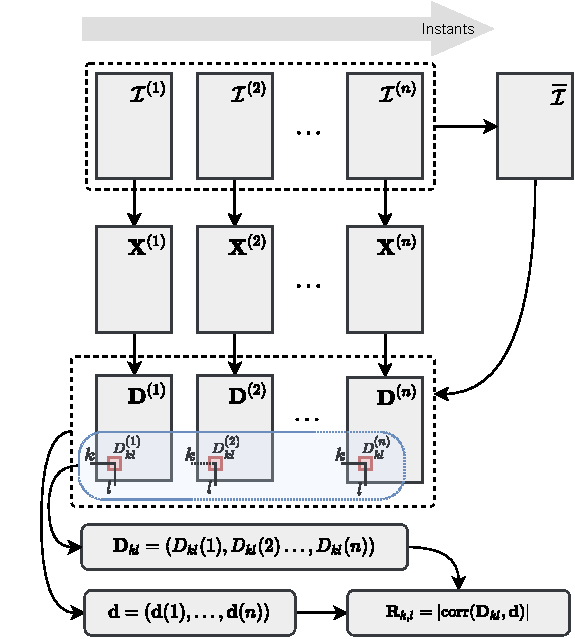
\includegraphics[scale=.8]{../../drawio/diagram_wecs.drawio_11nov21}
\caption{Diagram of steps performed on WECS to compute an absolute correlation of a single point.}
\label{figDiagram}
\end{figure}




Let $\mathcal{I}^{(1)},\ldots,\mathcal{I}^{(n)}$ be an image time series defined on a support $\mathcal{S} = \left\lbrace 1,\ldots,u  \right\rbrace \times \left\lbrace 1,\ldots,v  \right\rbrace \subset \mathbbm{N}^2$, hence representing a region of interest over $n$ distinct instants.
%
Such images are relative to one SAR channel or a combination of channels; this will be specified when appropriate. 
Our goal is twofold: to find possible points in time where some relevant changes might have taken place at the region represented in $\mathcal{I}^{(m)}$, $m=1,\ldots,n$, and to find which regions are closely associated to the observed changes over time. We shall address these tasks by analyzing the bidimensional stationary discrete wavelet decomposition of $\mathcal{I}^{(m)}$. Stationary wavelets (also known as non-decimated or redundant wavelets) is a traditional de-noising method that can be efficiently applied to two-dimensional signals such as images \cite{coifman1995translation,atto2012multidate,atto2016wavelet}. 


The application of this wavelet transform to $\mathcal{I}^{(m)}$ at some appropriate resolution level $J\geq 1$ results in a matrix of the so called approximation wavelet coefficients $\vX^{(m)}$ of $\mathcal{I}^{(m)}$ 
defined on the same support $\mathcal{S}$. The higher $J\in\{1,2,\ldots, \floor{ \log_2( \min\{u,v\} ) } \}$ is, the smoother $\vX^{(m)}$ gets.

Beyond many other aspects that are involved in wavelet analyses of images, which may include different wavelet bases as well as the use of thresholding of detail coefficients, the current construction is focused on $\vX^{(m)}$ to provide a simple wavelet smoothing. Nevertheless, extensions based on distinct aspects are straightforward.

We can then consider further apportioning the total $\mathbb{L}_2$ energy of the series $\left\{\vX^{(m)}\right\}_{m=1,\ldots,n}$ as:
\begin{equation}\label{E:eq_ANOVAlogimage}
\begin{split}
\sum_{m=1}^n\|\vX^{(m)}\|_F^2
= n\|\overline{\mathcal{I}}\|_F^2 + 2n\langle\overline{\vX}-\overline{\mathcal{I}},\overline{\mathcal{I}}\rangle_F + \\
+ \sum_{m=1}^n\|\mathcal \vX^{(m)} - \overline{\mathcal{I}}\|_F^2,
\end{split}
\end{equation}
where $\overline{\mathcal{I}}=n^{-1}\sum_{m=1}^n\mathcal{I}^{(m)}$ and $\overline{\vX}=n^{-1}\sum_{m=1}^n\vX^{(m)}$; $\| \cdot \|_F$ and $\left\langle \cdot , \cdot \right\rangle_F$ represents the Frobenius norm and inner product, respectively. Naturally, both $\overline{\mathcal{I}}$ and $\overline{\vX}$ share the support $\mathcal{S}$.


The last term on the right-hand side of Equation~(\ref{E:eq_ANOVAlogimage}) measures the deviations between the wavelet coefficients at distinct instants ($\vX^{(m)}; \ m=1,\ldots,n$) and the \textit{average image} (i.e., $\overline{\mathcal{I}}$). Such deviations may favor detecting relevant changes over time. Since each element (i.e., a pixel/position $(k,l)\in \mathcal{S}$) of $\vX^{(m)}$ also has a corresponding sequence of deviations in time, the local deviation to the overall measure may also allow detecting spatial changes. Among several approaches able to detect change events, the Pearson correlation coefficient is an interesting alternative. Furthermore, such measure shares connections with the idea of feature screening employed in high-dimensional regression \cite{fan2008sure}.


Let $X_{kl}^{(m)}$ and $\overline{\mathcal{I}}_{kl}$ be the entry $(k,l)$ of $\vX^{(m)}$ and $\overline{\mathcal{I}}$, respectively. 
%
The matrix $\vD^{(m)}$ embraces the squared differences between $\vX^{(m)}$ and $\overline{\mathcal{I}}$, where $D_{kl}^{(m)} = \left( \vX_{kl}^{(m)} - \overline{\mathcal{I}}_{kl} \right)^2$.
%
Therefore, the temporal overall variation sequence is defined as $\left\lbrace \vd^{(m)}  \right\rbrace_{m=1,\ldots,n}$, whose elements are given by:
\begin{equation}\label{E:eq_defdm}
\vd^{(m)} = \sum_{k=1}^{u} \sum_{l=1}^{v} D_{kl}^{(m)}.
\end{equation}


In this context, an instant $m$ in $\left\lbrace \vd^{(m)}  \right\rbrace_{m=1,\ldots,n}$ with high value stands for the image $\mathcal{I}^{(m)}$ where the most expressive changes take place.



In order to identify spatio-temporal changes, we employ the concept of ultra-high dimensional correlation screening \cite{fan2020statistical} discussed in Section~\ref{section_theroy}. For each local squared deviation time series given by individual elements of $\vD^{(m)}$ across $m=1,\ldots,n$, say $\vD_{kl} = \left\lbrace D_{kl}^{(1)},\ldots,D_{kl}^{(n)} \right\rbrace$, consider the absolute value of its Pearson correlation with the overall squared deviations $\vd$:
\begin{equation}\label{def_Rkld}
R_{kl}= |\corr \left( \vD_{kl}, \vd \right)|.
\end{equation}

Consequently, it is defined $\vR = \{R_{kl}\}$ as the matrix of absolute correlations, where $R_{kl}$ is assigned to each $(k,l) \in \mathcal{S}$.
%Let $\vR = \{R_{kl}\}$ be the matrix of absolute correlations, where $R_{kl}$ is assigned to each $(k,l) \in \mathcal{S}$.


Define a mapping of \textit{relevant} indices for changes over the image series with respect to $\overline{\mathcal I}$ as $\mathcal{M}^{\star} \subseteq \mathcal{S}$ where \textit{changes in $\{\mathcal{I}^{(m)}\}_{m=1,\ldots,n}$ with respect to $\overline{\mathcal{I}}$ are affected by local changes in the images}.



If we apply to Equation (\ref{E:eq_defdm}) the index dichotomy defined by $\mathcal{M}^\star$, we have
\begin{align}
\vd^{(m)}=\sum_{(k,l)}\beta_{kl}D_{kl}^{(m)}+\varepsilon^{(m)}, \label{Regressao}
\end{align}
where $\beta_{kl}$ are non-null regression coefficients for $(k,l)\in\mathcal{M}^\star$, and $\varepsilon^{(m)}$ are stochastic error terms. 
The error terms allow for both the apportionment of spurious correlation for indices not in $\mathcal{M}^\star$ as well as for the energies not represented by the wavelet smoothing.
 


It is a well-known property of discrete wavelet transforms that it statistically decorrelates the original data \cite{vidakovic1999statistical,morettin2017wavelets}. For instance, this motivates the use of WECS instead of a non-wavelet version of energy correlation, since wavelets will result in sparser representations for $\mathcal{M}^\star$. Moreover, the sure screening theoretical results for independent data motivates our conjecture that the regression set-up given by Equation (\ref{Regressao}) should have a good performance. A rigorous proof for dependent data sets such as multitemporal series of satellite images is beyond the scope of this manuscript, but the numerical results provide us with some solid evidences.


Finally, an empirical mapping of change locations may be stated as:
\begin{equation}
\mathcal{M}_{\tau} = \{(k,l) \in \mathcal{S} : |R_{kl}|>\tau\},
\label{E:def_Mtaud}
\end{equation}
where $\tau \in \mathbbm{R}_{+}^{*}$ is a convenient threshold value. The idea is that, for suitable values of $\tau$, the empirical set $\mathcal{M}_{\tau}$ has high probability of detecting the correct change locations in $\mathcal{M}^{\star}$ \cite{fan2020statistical}.




%%%%%%%%%%%%%%%%%%%%%%%%%%%%%%%%%%%%%%%%%%
\section{Experiments}\label{secExperiments}

%%%%%%%%%%%%%%%%%%%%%
\subsection{Experimental design}\label{secExpDesign}

In order to assess the proposed method's performance, this section presents two studies comprising distinct datasets.

The first study (Sec.~\ref{secExpSimulated}) uses a simulated data set and focus on identifying the most appropriate wavelet family and resolution level $J$. Specifically, the Haar (haar), Daubechies of order 2 and 4 (db2 and db4), Coiflets of order 4 (coif4) and Symlets of order 2 and 4 (sym2 and sym4) wavelet families are analyzed \cite{BeylkinEA1991,Daubechies1992}. 
The performance of the proposed method is measured in terms of True/False Positive Ratios and Receiver Operating Characteristic (ROC) curve. 


Comparisons with the standard Thresholding of Aggregate Absolute Difference (TAAD) and a non-wavelet version of WECS, herein called Energy Correlation Screening (ECS), are included in the experiments. 
In summary, the TAAD comprises the application of a thresholding algorithm on the accumulated change representation image $\vA$ where $A_{kl} = \sum_{m=2}^{n}|\mathcal{I}_{kl}^{(m)}-\mathcal{I}_{kl}^{(m-1)}|$. 
The ECS stands for the use of $\mathcal{I}^{(m)}$ instead of $\vX^{(m)}$ when defining $D_{kl}^{(m)}$ at Equation~\ref{E:eq_defdm}, and consequently Equation~\ref{def_Rkld}. The resulting ``Pearson correlation'' matrix from ECS approach is denoted by $\widetilde{\vR}$.


The second study (Sec.~\ref{secExpActual}) presents an analysis on the performance of WECS, and respective comparison with TAAD and ECS, in a real-world application with actual SAR image series. The appropriate wavelet family and resolution level previously identified are employed. 
F1-Score \cite{Rijsbergen1979}, True/False Positive/Negative (TP, TN, FP and FN) rates, the kappa coefficient, and the variance of kappa \cite{Congalton2019}, are adopted for this purpose. Additionally, the computational run-times are presented and discussed.



We used a computer with an Intel Intel i-7 processor (\SI{8}{core}, \SI{3.5}{\giga\hertz}), and \SI{16}{\giga\byte} of RAM running the Ubuntu Linux version~20.04 operating system.
The code of the proposed method is freely available at \url{https://github.com/rodneyfv/wecs}. 


%%%%%%%%%%%%%%%%%%%%
\subsection{Simulated data analysis}\label{secExpSimulated}

We discuss here the application of  WECS, TAAD, and ECS on a simulated multi-temporal image dataset. 
Such series comprises 80 multi-temporal images and it is synthesized by repeating a sequence of four images with different types of changes plus noise. 
Examples of the first four time instants are shown in Figure~\ref{F:EllipsoidChanges}. 
These images/instants are generated by summing two matrices: (i) a binary signal matrix with ones denoting where the ellipses occur and zero elsewhere; (ii) and a noise matrix with random variables following a standard Gaussian distribution. 

The first image, $\mathcal{I}^{(1)}$, presents three elongated ellipses. The second image $\mathcal{I}^{(2)}$ has shorter and larger ellipses added. Smaller ellipses are then added to form $\mathcal{I}^{(3)}$ and $\mathcal{I}^{(4)}$. Patterns of changes between subsequent images are shown in Figure~\ref{figResSim1}, where white regions (i.e., ``ones'') correspond to changes.

Applying WECS to these images we obtain a matrix $\vR$ of correlations between deviations of each $\mathcal{I}$ entry with the total squared mean deviation. A typical example of $\vR$ is presented in Figure~\ref{figResSim2}. For some choice of threshold $\tau$ on absolute values of $\vR$, we obtain a binary matrix that can be compared with the total true changes shown in Figure \ref{figResSim1}.
Similarly, Figures~\ref{figResSim3} and \ref{figResSim4} depict the matrices $\vA$ and $\widetilde{\vR}$ provided by TAAD and ECS methods.



%-----------------------
\begin{figure}[hbt]
\centering

\mbox{
\subfigure[$\mathcal{I}^{(1)}$]{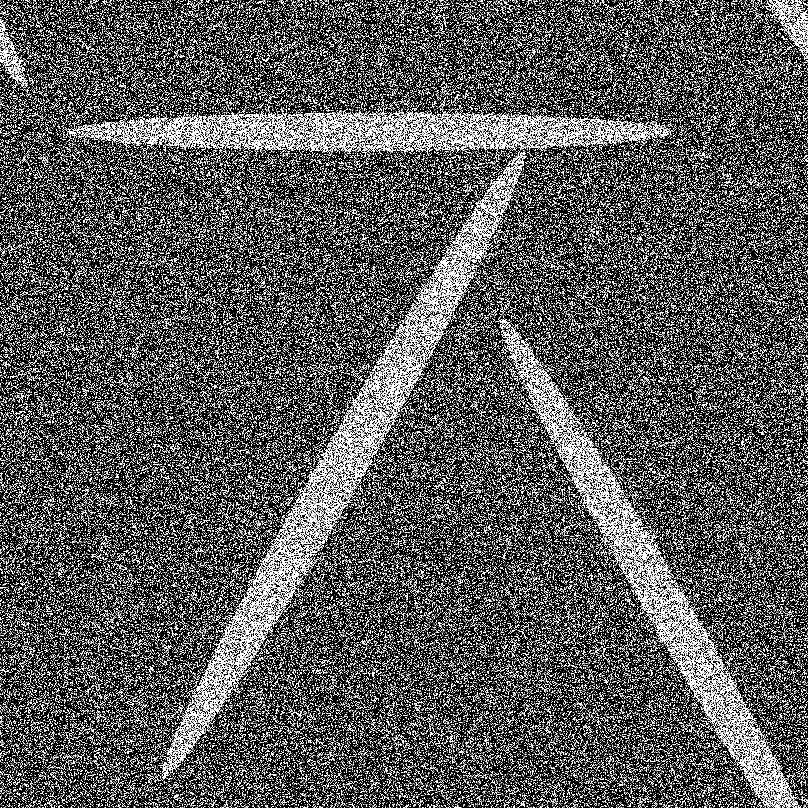
\includegraphics[width=0.23\textwidth]{../../figs/ellipses_t1_adjust.png}\label{figSim1}} 
\subfigure[$\mathcal{I}^{(2)}$]{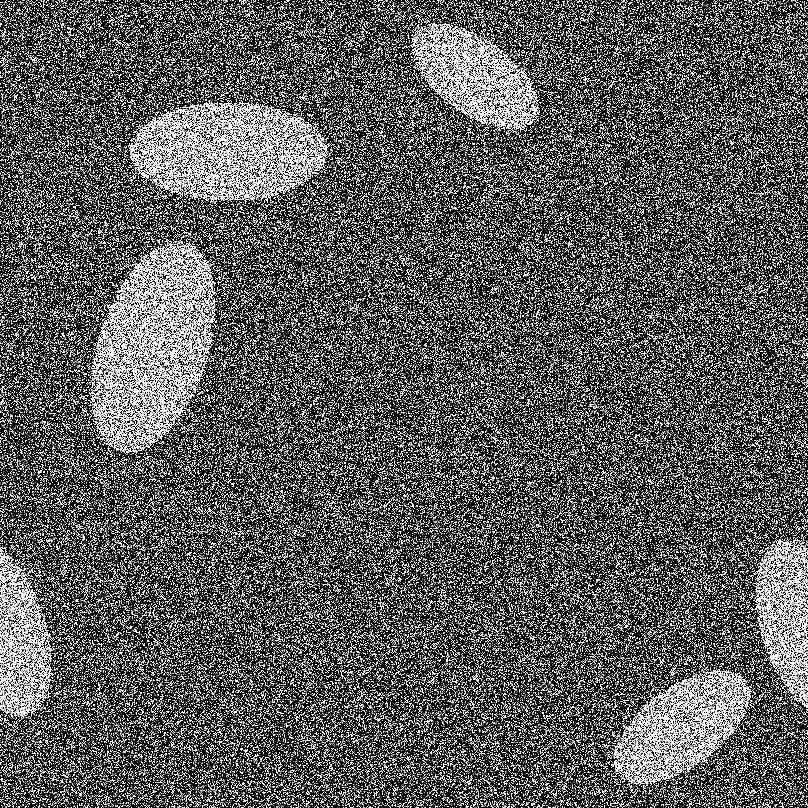
\includegraphics[width=0.23\textwidth]{../../figs/ellipses_t2_adjust.png}\label{figSim2}}
}
\mbox{
\subfigure[$\mathcal{I}^{(3)}$]{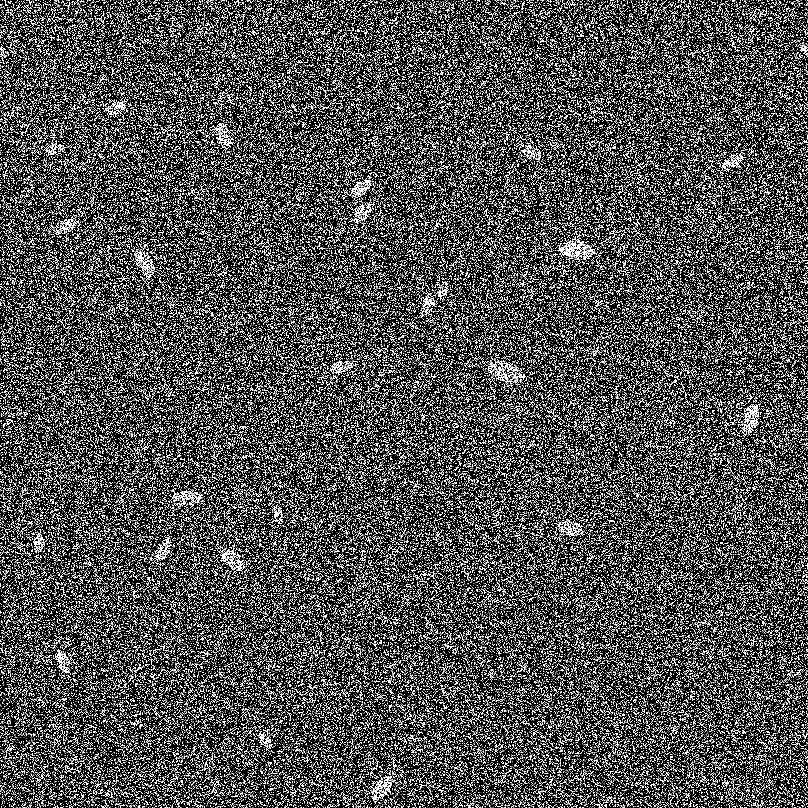
\includegraphics[width=0.23\textwidth]{../../figs/ellipses_t3_adjust.png}\label{figSim3}} 
\subfigure[$\mathcal{I}^{(4)}$]{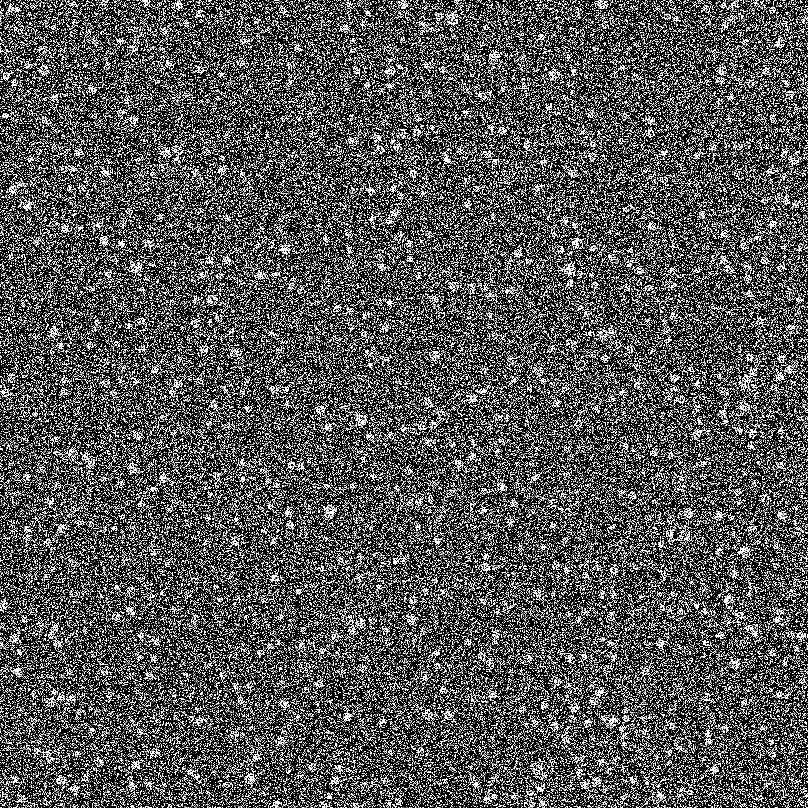
\includegraphics[width=0.23\textwidth]{../../figs/ellipses_t4_adjust.png}\label{figSim4}}
}

\caption{Example of the first four simulated multi-temporal images. Features and changes come as white ellipses and dots.}
\label{F:EllipsoidChanges}
\end{figure}



%-----------------------
\begin{figure}[hbt]
\centering

\mbox{
\subfigure[Total changes]{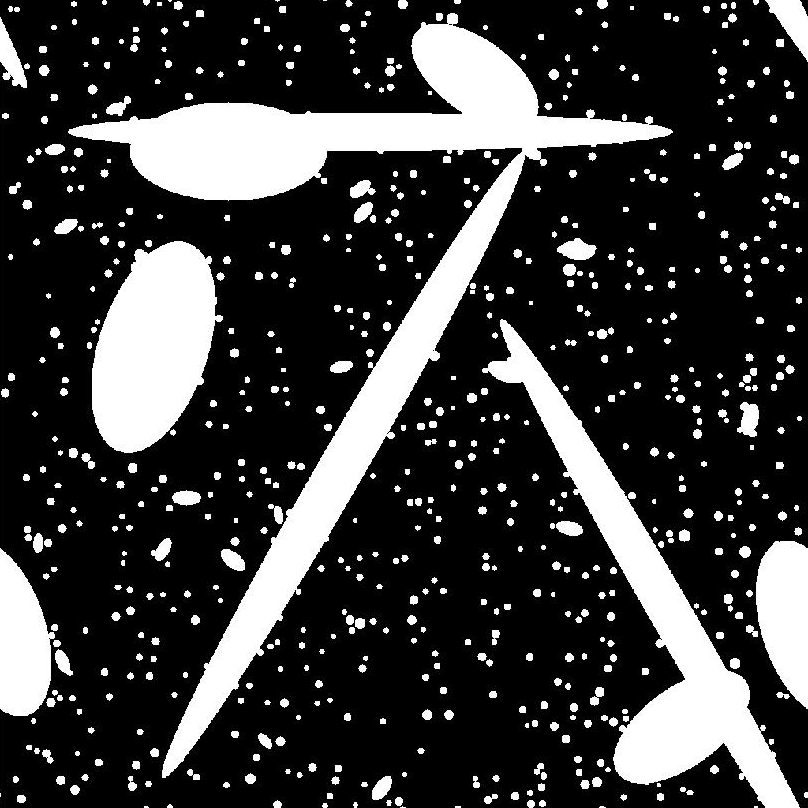
\includegraphics[frame,width=0.23\textwidth]{../../figs/total_changes_adjust.png}\label{figResSim1}} 
\subfigure[WECS (db2, $J=2$) -- $\vR$]{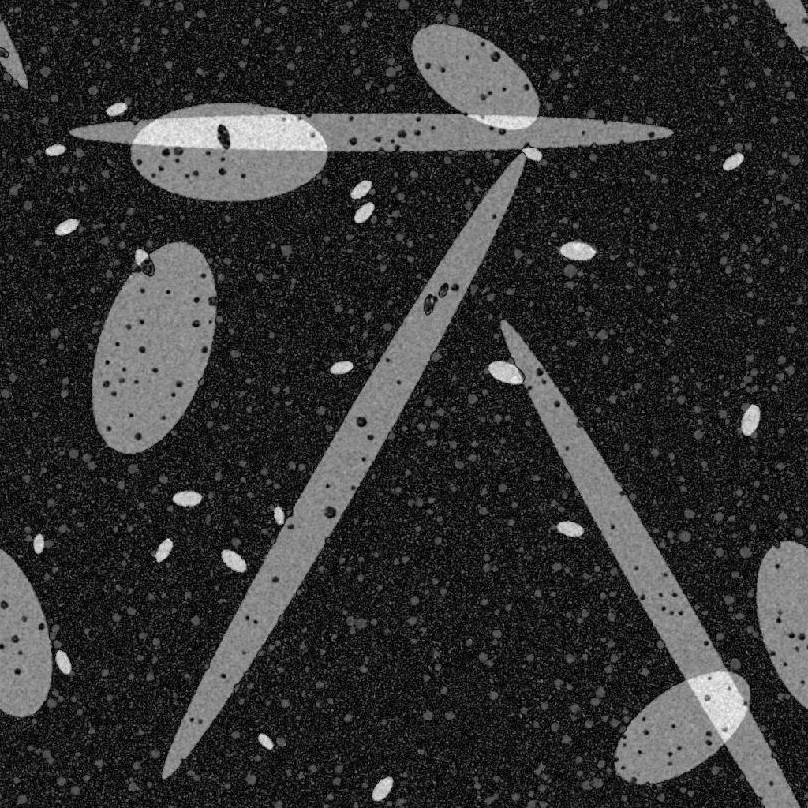
\includegraphics[frame,width=0.23\textwidth]{../../figs/corr_changes_dm_adjust.png}\label{figResSim2}} 
}
\mbox{
\subfigure[TAAD -- $\vA$]{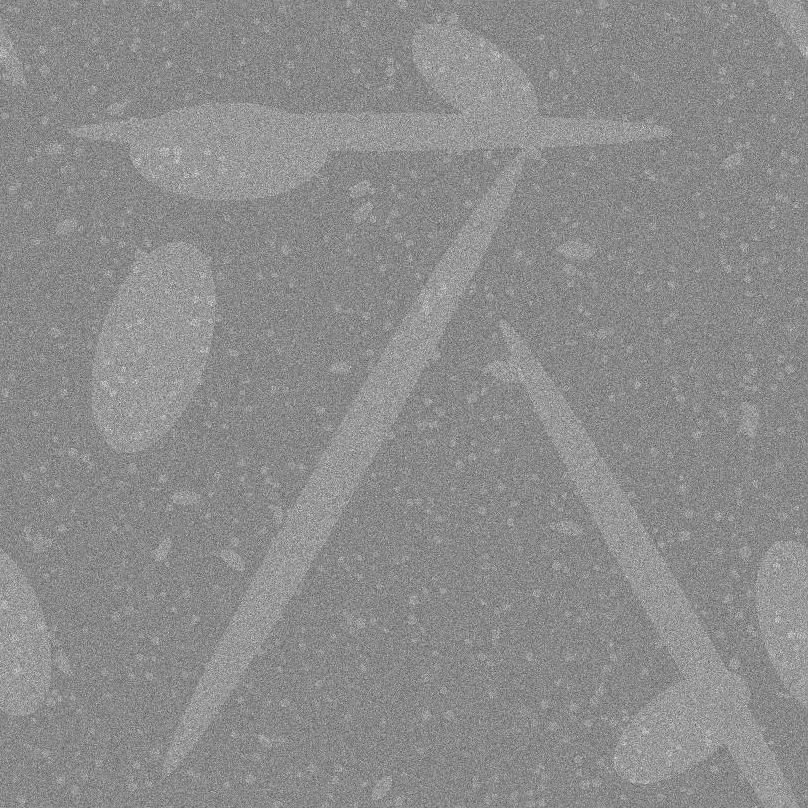
\includegraphics[width=0.23\textwidth]{../../figs/corr_changes_logratios_adjust.png}\label{figResSim3}} 
\subfigure[ECS -- $\widetilde{\vR}$]{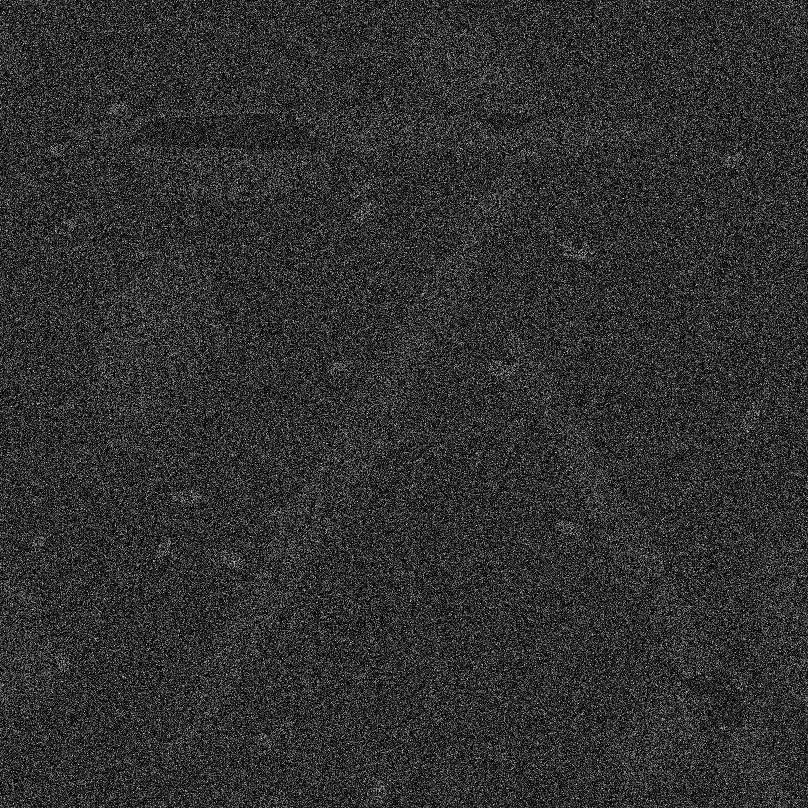
\includegraphics[frame,width=0.23\textwidth]{../../figs/corr_changes_dm_nowavelets_adjust.png}\label{figResSim4}} 
}

%\caption{Simulated images with changing ellipses. (a) Image composed by the total changes over time. (b) Proposed db2 WECS $\vd(m)$ with $J=2$; (c) Standard approach. (d) $\vd(m)$ without wavelets.}
\caption{Expected change/non-change regions and typical results provided by WECS, TAAD and ECS before the thresholding process.}
\label{F:Changes_methods_images}
\end{figure}



According to the experimental design (Section~\ref{secExpDesign}), ROC curves are employed to compare the performance of each analyzed method and inspect the effects of both $J$ and wavelet basis on the performance of the WECS method. In summary, the ROC curves exhibit the performance as a function of true and false positive ratios when distinguishing two events (in this context, the change and no-change pixels/positions) using distinct thresholds. The true and false positive ratios are computed using the ``total change'' image (Fig.~\ref{figResSim1}) as reference. Moreover, the tested thresholds embrace all values in $\vR$ (or $\vA$), excluding repetitions and considering it in ascending order.



%-----------------------
\begin{figure}[hbt]
\centering

\mbox{
\subfigure[WECS with different wavelet bases and J=2]{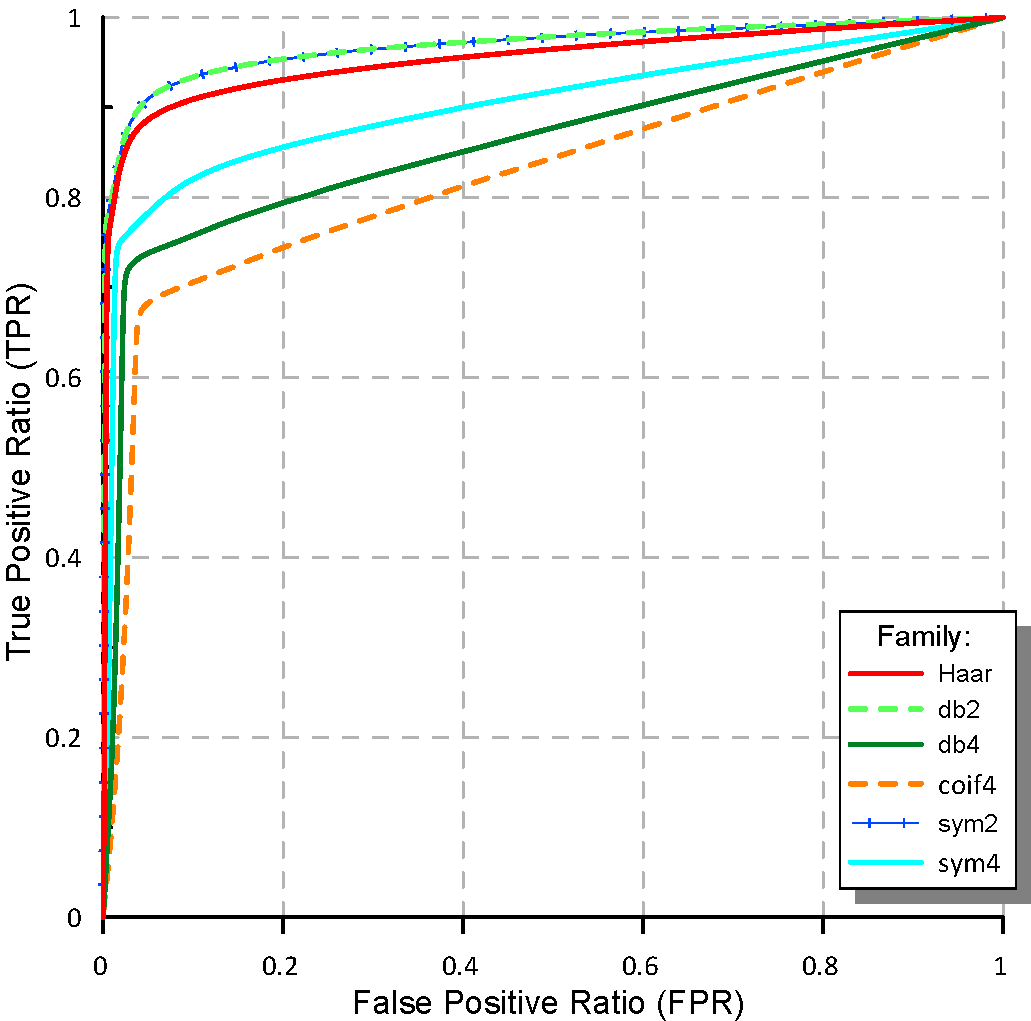
\includegraphics[width=0.23\textwidth]{../../graphs/basisROC.pdf}\label{figROCSimBasis}} \quad
\subfigure[WECS with db2 basis and different decomposition levels]{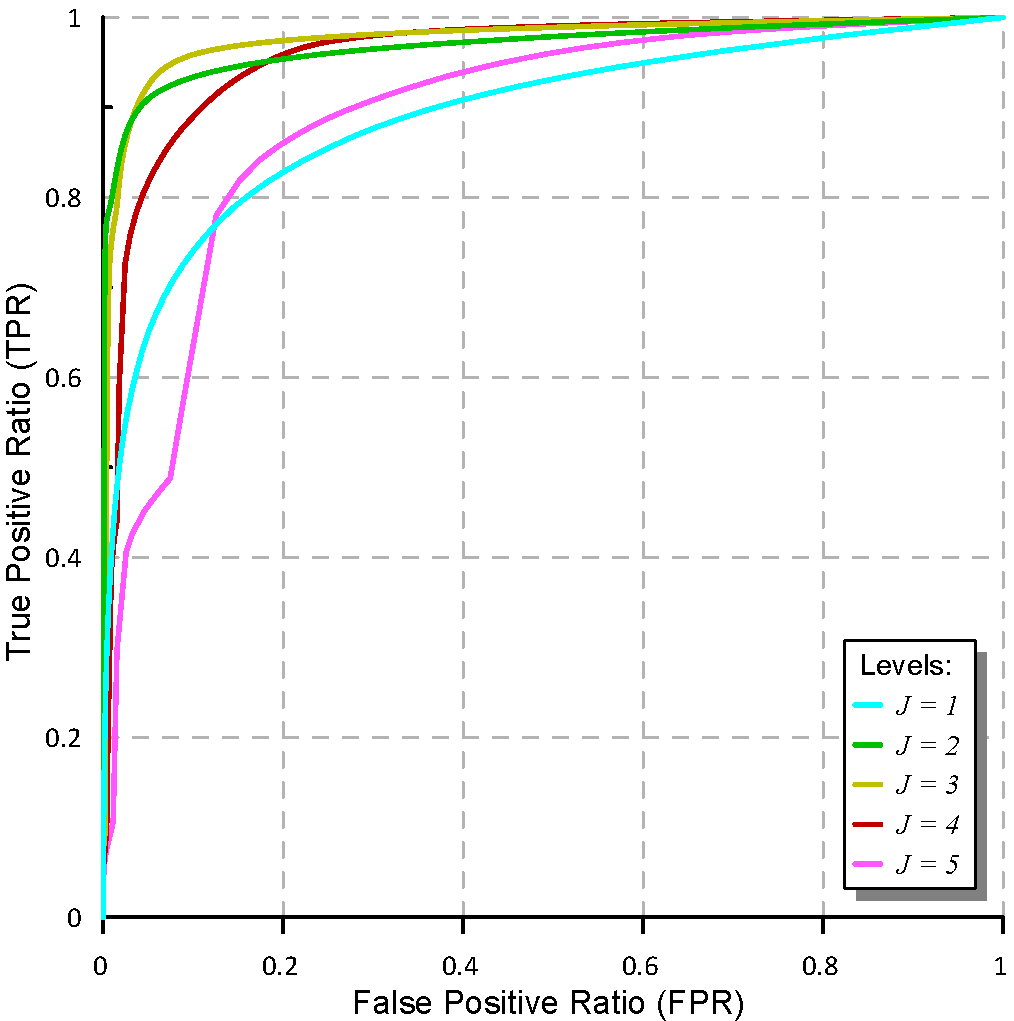
\includegraphics[width=0.23\textwidth]{../../graphs/levelsROC.pdf}\label{figROCSimJ}}
}

\mbox{
\subfigure[ROC curve comparison between WECS (db2 and $J=2$), TAAD and ECS methods]{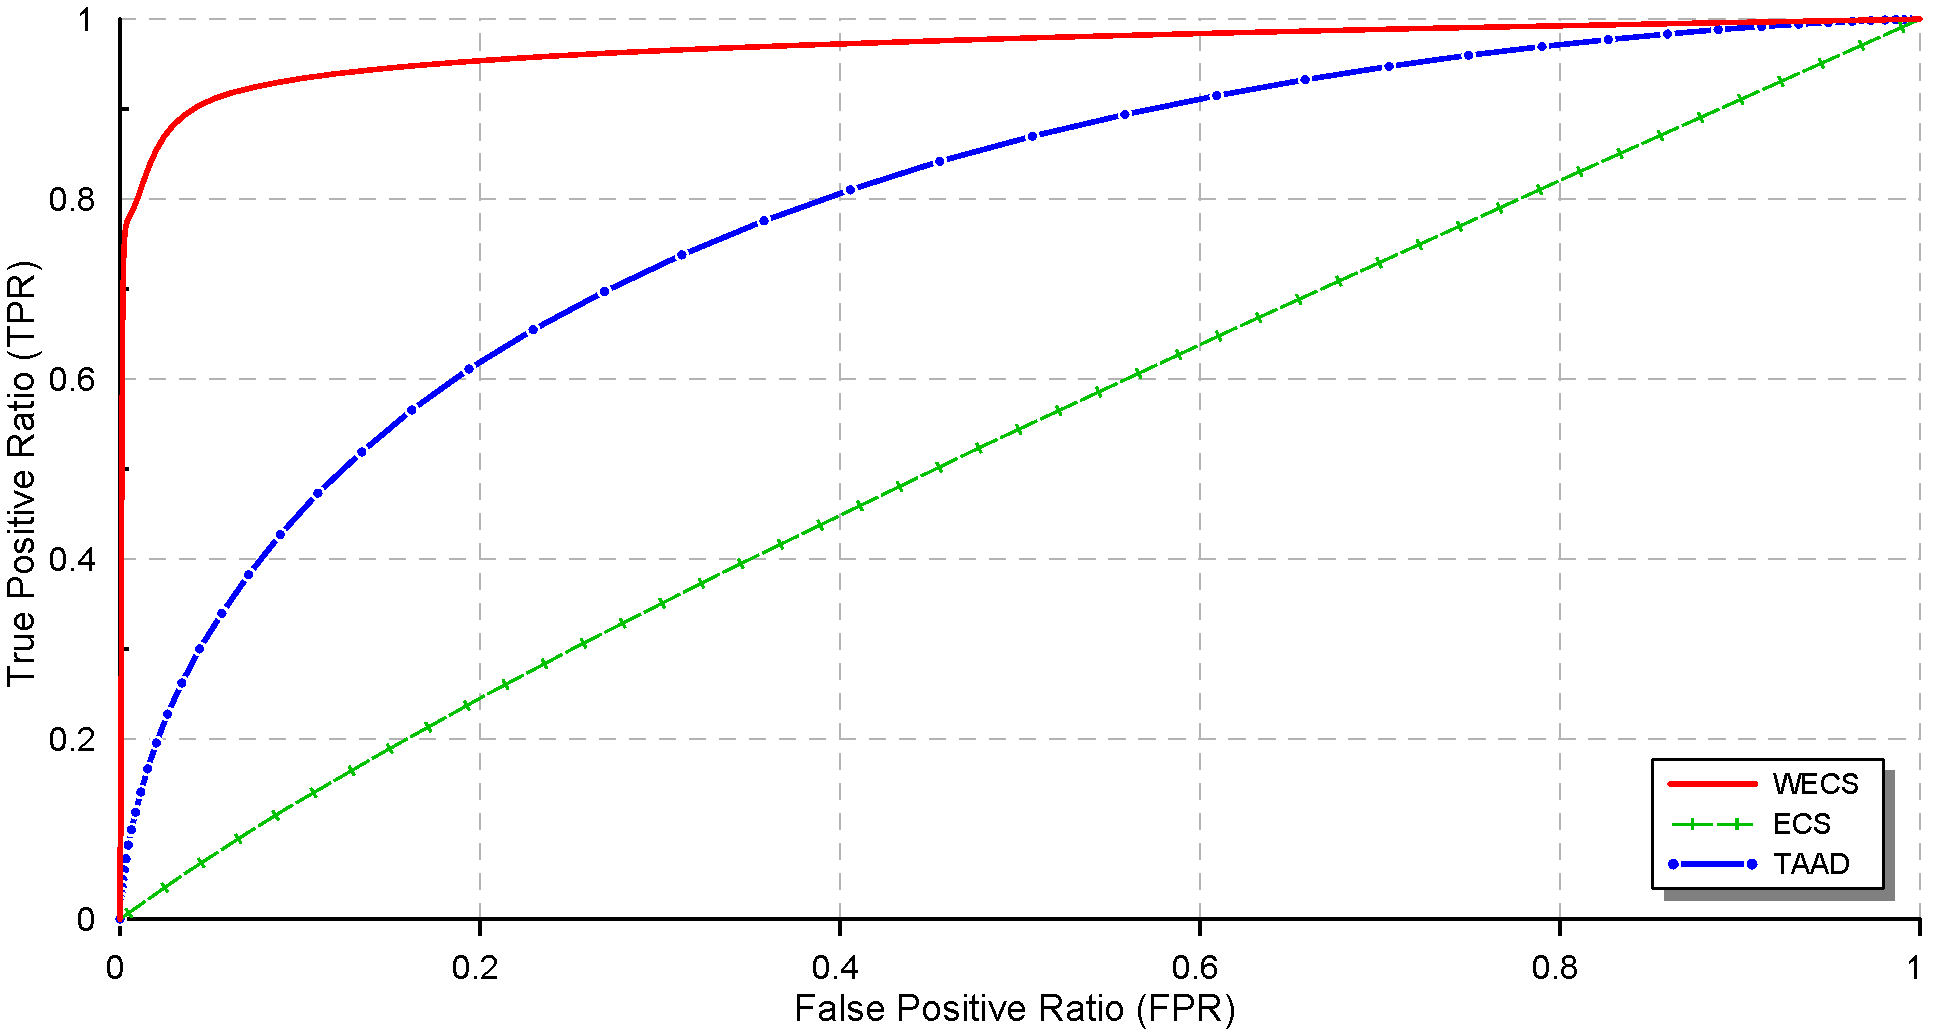
\includegraphics[width=0.46\textwidth]{../../graphs/methodROC_ext.pdf}\label{figROCSimRes}}
}

\caption{ROC curves related to the experiment with simulated dataset.}\label{F:EllipsoidChanges_details}
\end{figure}



%basis wavelet
Figure~\ref{figROCSimBasis} presents the ROC curves considering different wavelet bases in the WECS method. All instances adopt $J=2$. We conclude that db2 and sym2 deliver the best trade-off between true and false positive ratios (i.e., high true positive ratios even when the false positive ratios are low).
As a consequence of this finding, all the following experiments and analyses consider the db2 wavelet basis.

%J-level
Figure~\ref{figROCSimJ} depicts the ROC curves with $J \in \{1,2,3,4,5\}$ as decomposition levels. The profiles exhibited by the ROC curves provide evidences that $J$ equal to 2 or 3 lead to the best performances.  $J=2$ has a slight advantage, since it demands fewer decomposition levels. The overall performance for $J=2$ warrants its use for the rest of the comparisons.

%Compara figA
The ROC curves shown in Figure~\ref{figROCSimRes} present the performances of WECS, TAAD and ECS. 
ECS's low performance shows that the simple swap of the wavelet transform by a ``deviation image'' into the proposed correlation screening pipeline is an inconvenient choice and reinforces the importance of the wavelet smoothing in the context of the proposed method.
Regarding TAAD's performance, a True Positive Ratio of 0.8 is guaranteed when tolerating a False Positive Ratio of approximately 0.4. 
Since WECS provides the same True Positive Ratio under an almost nil false positive ratio, its superior performance is clearly established.


%%%%%%%%%%%%%%%%%%%%
\subsection{Actual remote sensing application}\label{secExpActual}


This section compares the performance of WECS, TAAD and ECS in a real-world change detection application. The appropriate wavelet basis and resolution level previously identified in Section~\ref{secExpSimulated} (i.e., db2 and $J=2$) are employed.

We consider here a large multi-temporal series of 85 images acquired over a forest region at the border of Brazil and the French Guiana (Fig.~\ref{figAE}), from December 26th 2015 to December 3rd 2017, by the SAR sensor onboard the Sentinel-1 satellite.


Each image contains the amplitude signal backscatters relative to VV and VH polarizations, a spatial resolution of \SI{10}{\meter} and a support of $1538 \times 1556$ pixels wide in ground range projection. 
Specifically, these images where obtained from the \textit{Sentinel-1 SAR GRD} dataset maintained by the European Space Agency \cite{ESA2021}.
%
Figures~\ref{figImgSentinel2015} and \ref{figImgSentinel2017} depict the first and last images of the time series, where it is possible to compare and identify some landscape changes.

After careful visual inspection of the backscatter profile of each image in the series, it is possible to identify the regions where the land cover change occurs or does not occur, allowing then collecting reference samples regarding the ``change'' and ``non-change'' conditions. 
Such samples are needed to compute the accuracy measures beforehand mentioned in Section~\ref{secExpDesign}. The spatial distribution of these samples is presented in Figure~\ref{figImgSentinelROIs}.


%-----------------------
\begin{figure}[hbt]
\centering
\includegraphics[width=0.485\textwidth]{../../qgis/maps/StudyArea_OSM.pdf}
\caption{The study area location.}\label{figAE}
\end{figure}


%-----------------------
\begin{figure}[hbt]
\centering

\mbox{
\subfigure[December 26th 2015]{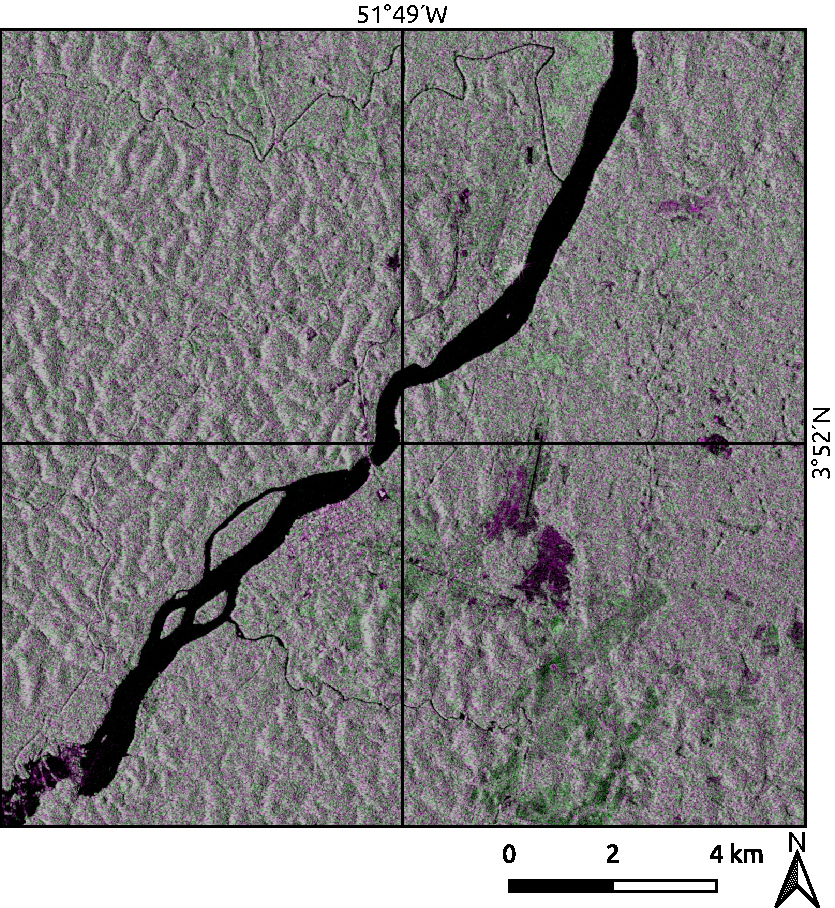
\includegraphics[width=0.23\textwidth]{../../qgis/maps/Sentinel_2015.pdf}\label{figImgSentinel2015}} 
\subfigure[December 3rd 2017]{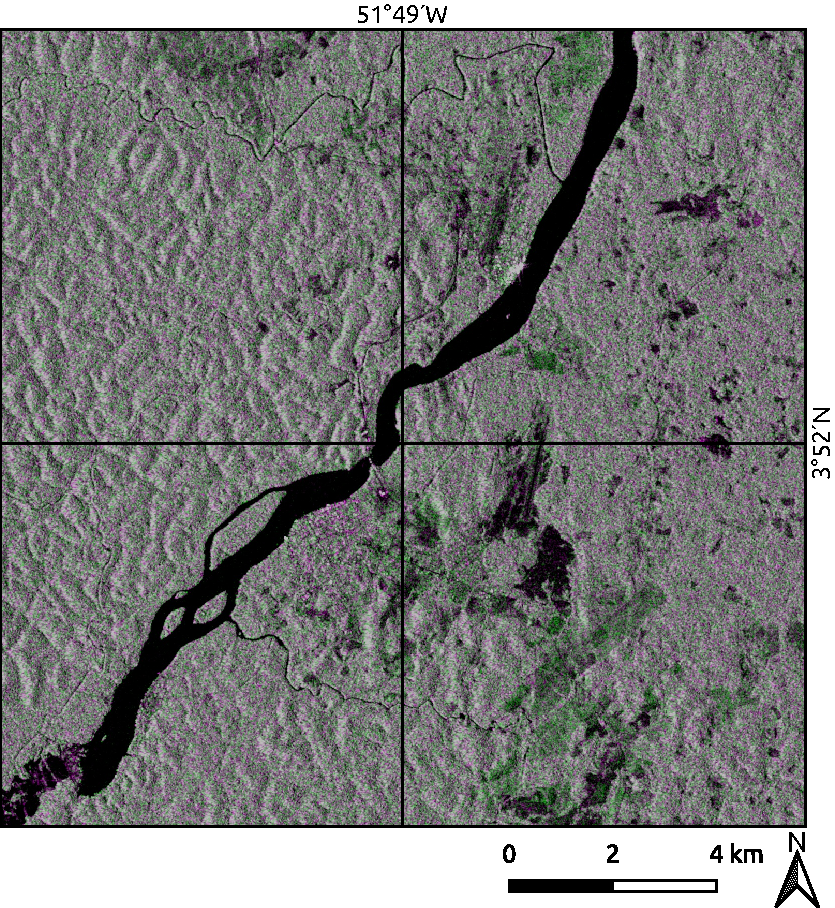
\includegraphics[width=0.23\textwidth]{../../qgis/maps/Sentinel_2017.pdf}\label{figImgSentinel2017}}
}

\subfigure[Reference change and non-change samples]{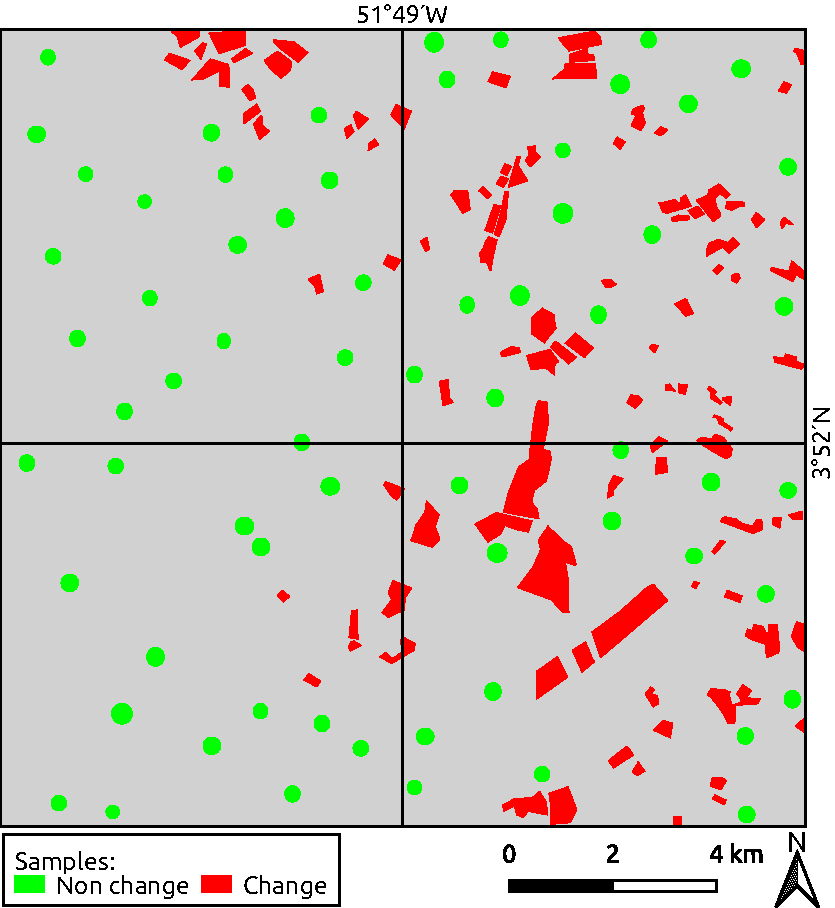
\includegraphics[width=0.23\textwidth]{../../qgis/maps/SamplesRev.pdf}\label{figImgSentinelROIs}}

\caption{First and last images in the adopted multitemporal image series, in VV-HV-VV RGB color composition, and reference samples.}\label{figImageRef}
\end{figure}


In order to apply the analyzed methods, the dual-polarized images were combined into a single-band representation considering the so-called "span" image
$\mathcal{I}_{kl}^{(m)} = \sqrt{(\mathrm{VV}_{kl}^{(m)})^2+(\mathrm{VH}_{kl}^{(m)})^2}$, with $\mathrm{VV}$ and $\mathrm{VH}$ representing the available polarizations.


Initially, to express the instantaneous change values with respect to WECS,
Figure~\ref{F:forest_wecs} presents the temporal variations given by $\vd$. According to the presented profile, it is possible to observe the fluctuations around a central value near $12$ as highlight instants with a value similar, higher or lower than this baseline, as pointed out for $m$ equal to 1, 30 and 59, respectively.
%
For the sake of comparison, the wavelet representation at each mentioned instant (i.e., $\vX^{(1)}$, $\vX^{(30)}$ and $\vX^{(59)}$) and the mean image (i.e., $\overline{\mathcal{I}}$) are exhibited in Figure~\ref{F:forest_change_times}. While $\vX^{(1)}$ shares similarities with $\overline{\mathcal{I}}$, evident changes increase in $\vX^{(30)}$. Reversely, $\vX^{(59)}$ offers low contribution for identifying change regions.



%-----------------------
\begin{figure}[htb!]
\centering
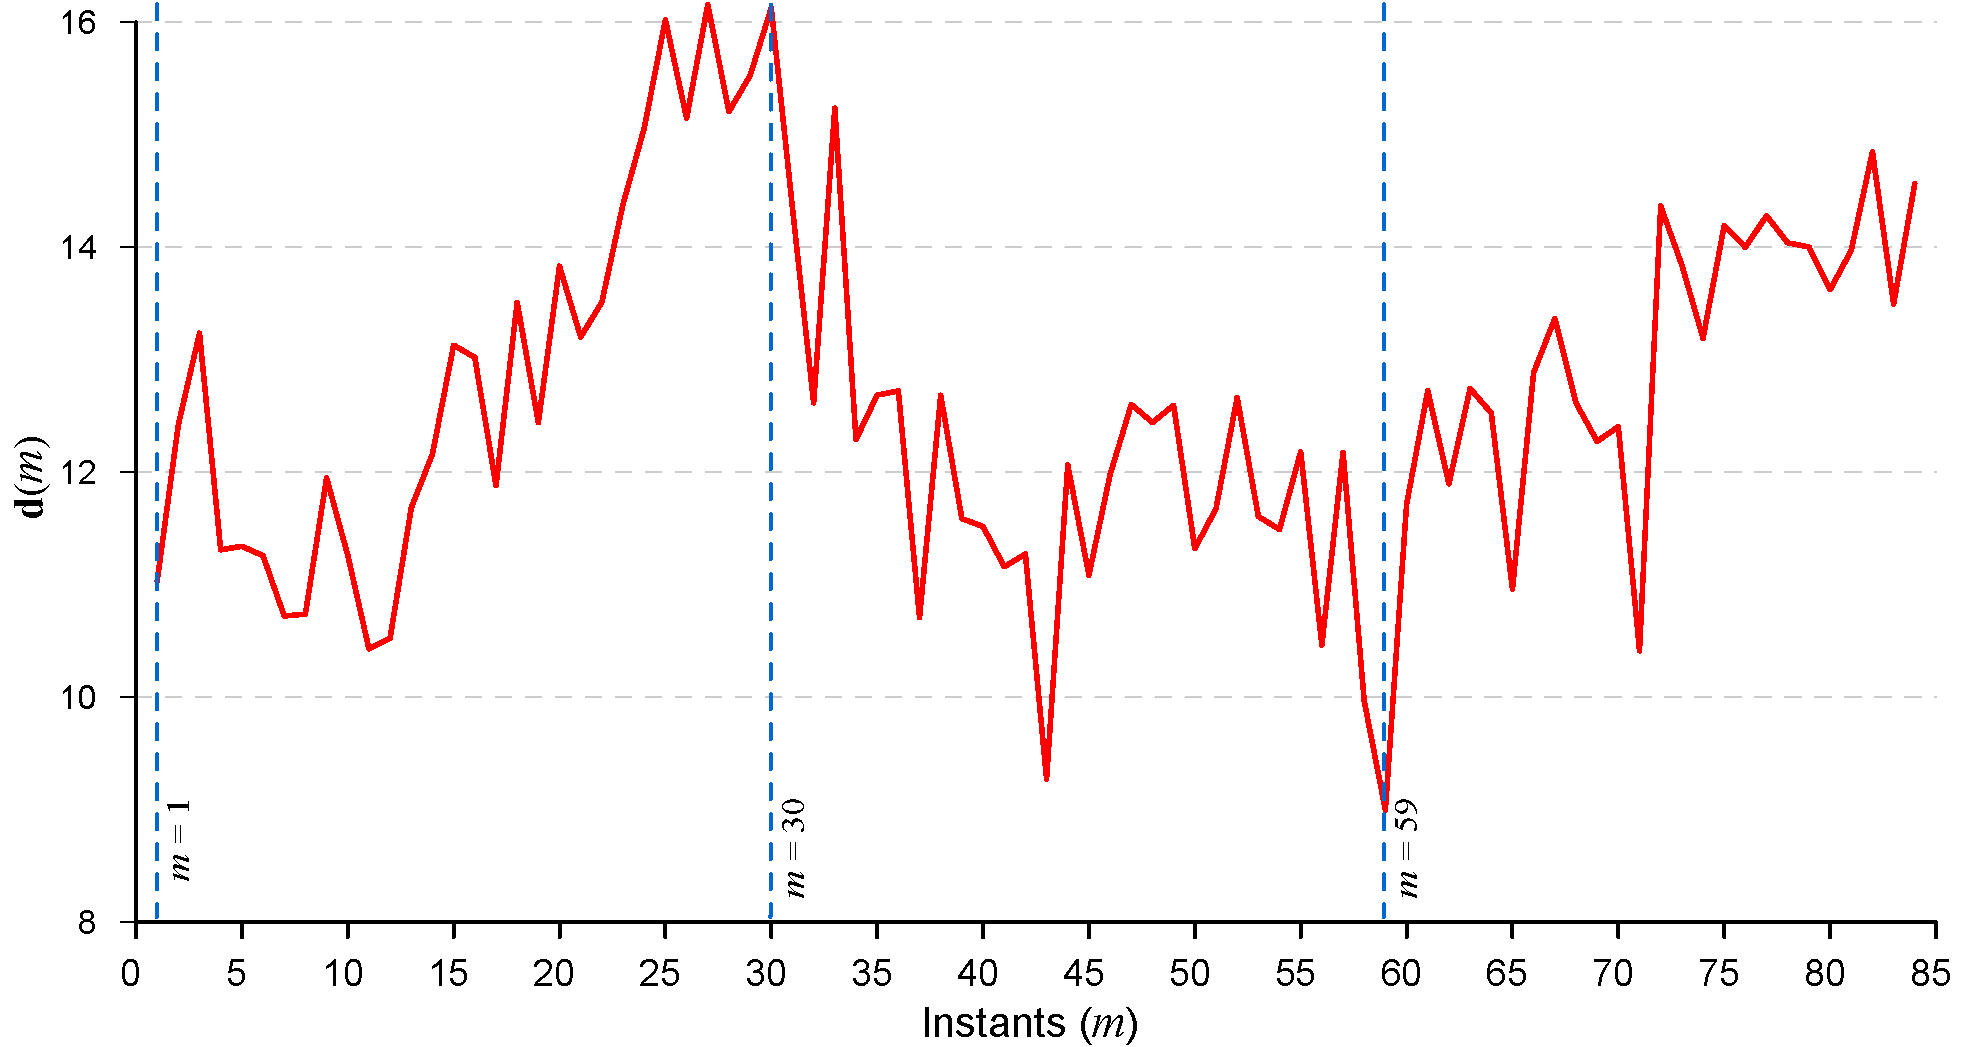
\includegraphics[width=0.485\textwidth]{../../graphs/LineInstants_1-30-59.pdf}
\caption{Plot of $\vd(m)$ for $m=1,\ldots,85$. Distinct deviations occur at $m=1$ (intermediate), $30$ (high) and $59$ (low). Baseline around 12.}\label{F:forest_wecs}
\end{figure}



%-----------------------
\begin{figure}[hbt]
\centering

\mbox{
\subfigure[$m=1$]{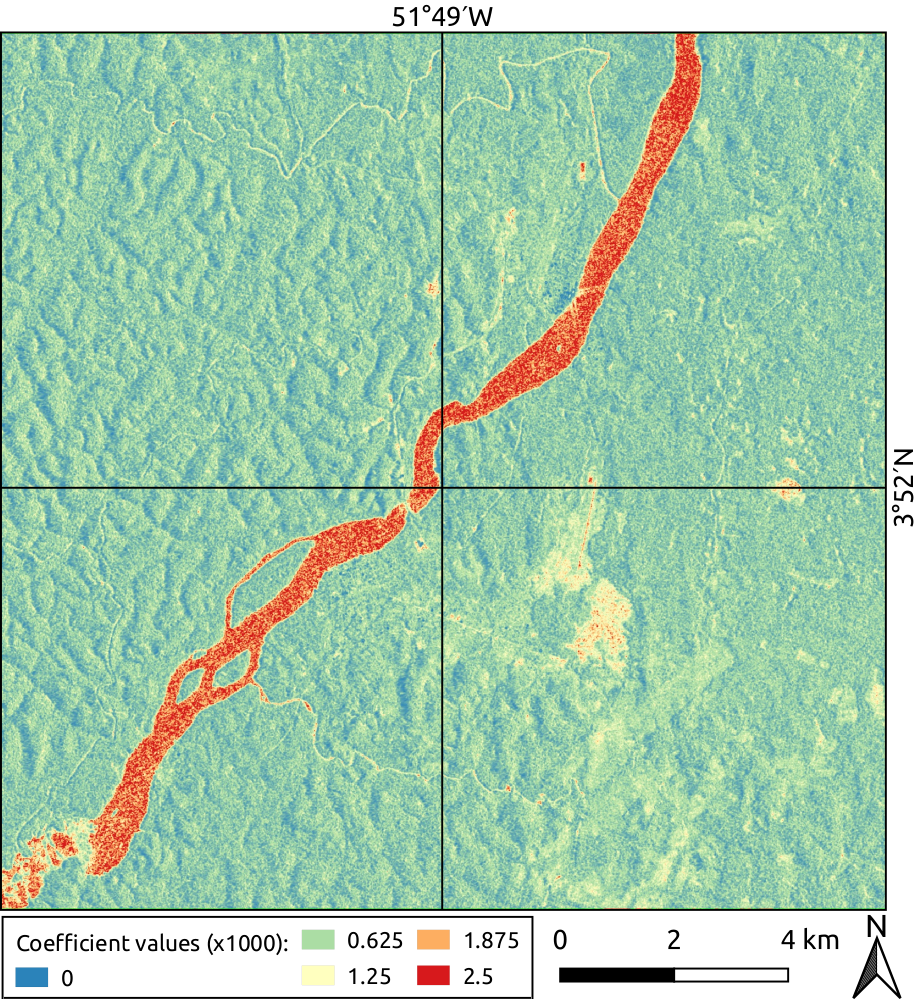
\includegraphics[width=0.23\textwidth]{../../qgis/maps/X_1.png}\label{maps_X_1}} 
\subfigure[$m=30$]{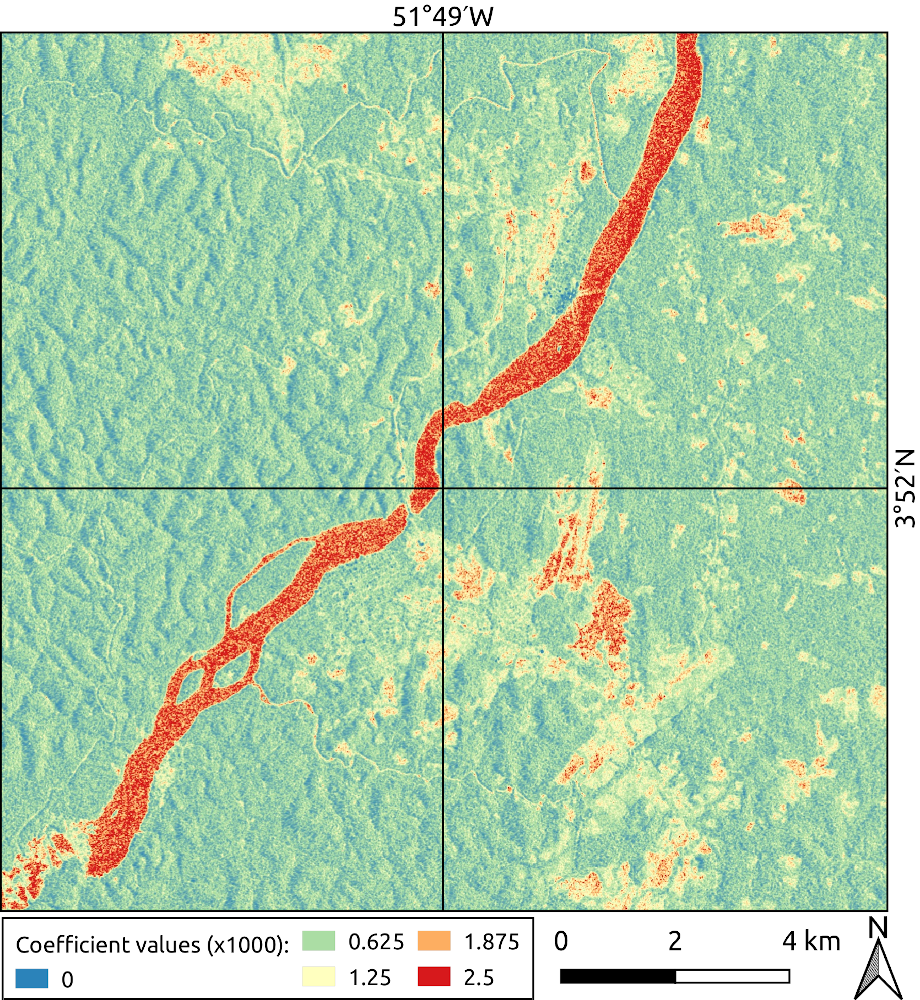
\includegraphics[width=0.23\textwidth]{../../qgis/maps/X_30.png}\label{maps_X_30}}
}

\mbox{
\subfigure[$m=59$]{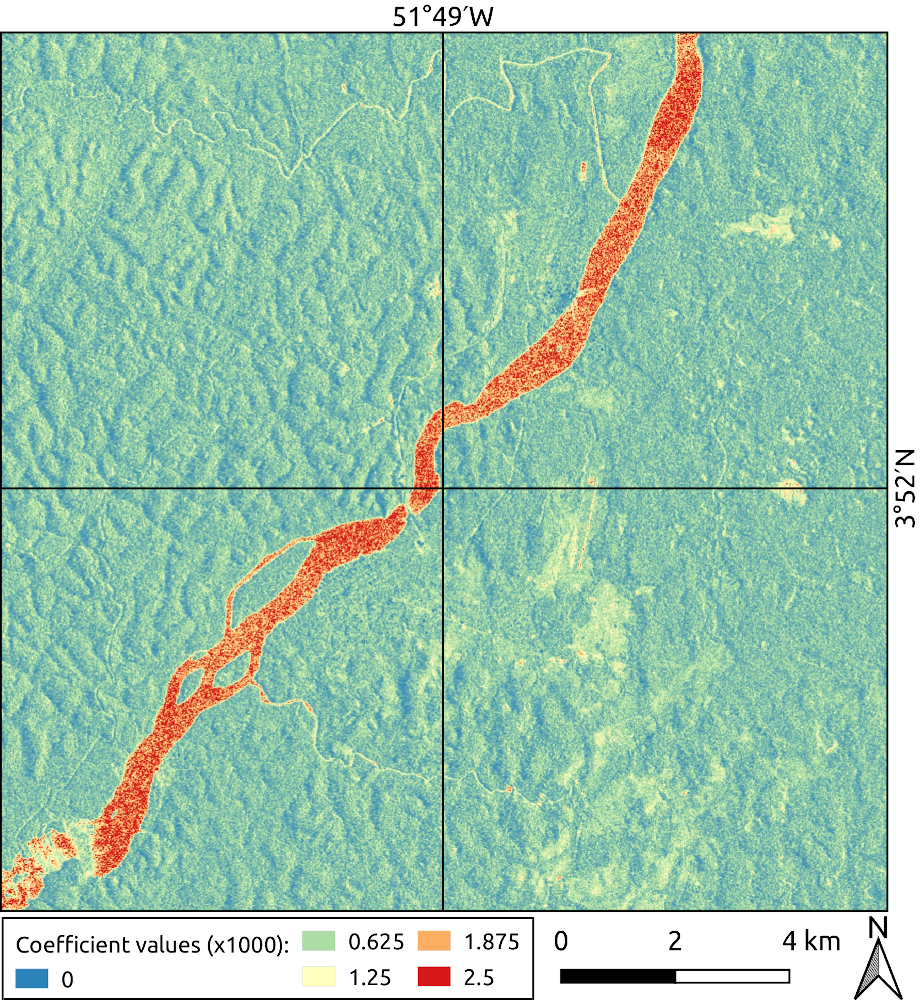
\includegraphics[width=0.23\textwidth]{../../qgis/maps/X_59.png}\label{maps_X_59}} 
\subfigure[$\overline{\mathcal{I}}$]{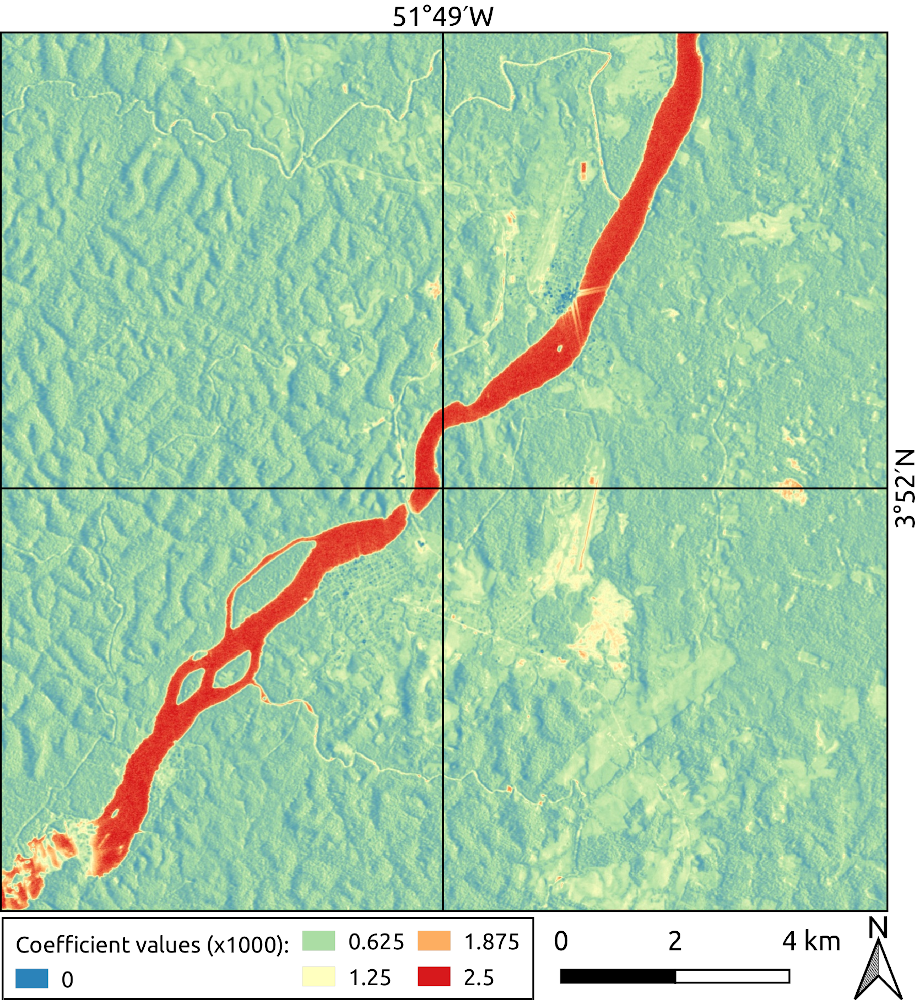
\includegraphics[width=0.23\textwidth]{../../qgis/maps/X_mean.png}\label{maps_X_mean}}
}

\caption{Images $\vX^{(m)}$ for $m=1,30,59$ and mean image $\overline{\mathcal{I}}$.}
\label{F:forest_change_times}
\end{figure}



%After submitting the image series to the methods WECS, ECS and TAAD, are obtained the matrices $\vR$, $\widetilde{\vR}$ and $\vA$, respectively, comprising measure about a tendency of changes in each position of the spatial domain.
Through the application WECS, ECS and TAAD to the image series, we obtain matrices $\vR$, $\widetilde{\vR}$ and $\vA$. They represent the spatially-localized change measures given by WECS, ECS and TAAD, respectively. Such matrices are presented in Figure~\ref{figImageMethods}, where high values stand for regions with changes in their land cover over time.
%
However, to determine a cut-off value $\tau$ for such matrices, providing then binary maps $\mathcal{M}_{\tau}$ of ``change'' and ``non-change'' areas (Equation~\ref{E:def_Mtaud}), the use of thresholding techniques rises as a convenient procedure. 
Among different alternatives in the literature, the Otsu (OT) \cite{otsu1979threshold} and Kittler-Illingworth (KI) \cite{KittlerIllingworth1986} thresholding techniques had been successfully employed for change detection purposes \cite{JohnsonKasischke1998,Nielsen2007,WuEA2014,NegriEA2021}.


The accuracy of the binary maps $\mathcal{M}_{\tau}$, resulting from the application of OT and KI algorithms on the change images provided by WECS, ECS and TAAD, are measured in terms of the F1-Score and the kappa coefficient based on the reference ground-truth samples (Fig.~\ref{figImgSentinelROIs}). 
Table~\ref{tabAccExpSentinel} presents the computed accuracy measures.
%Moreover, the percentages of True and False Positives and Negatives are shown in Figure~\ref{figTPTNs}.



%-----------------------
\begin{figure}[hbt]
\centering

\mbox{
\subfigure[WECS -- $\vR$]{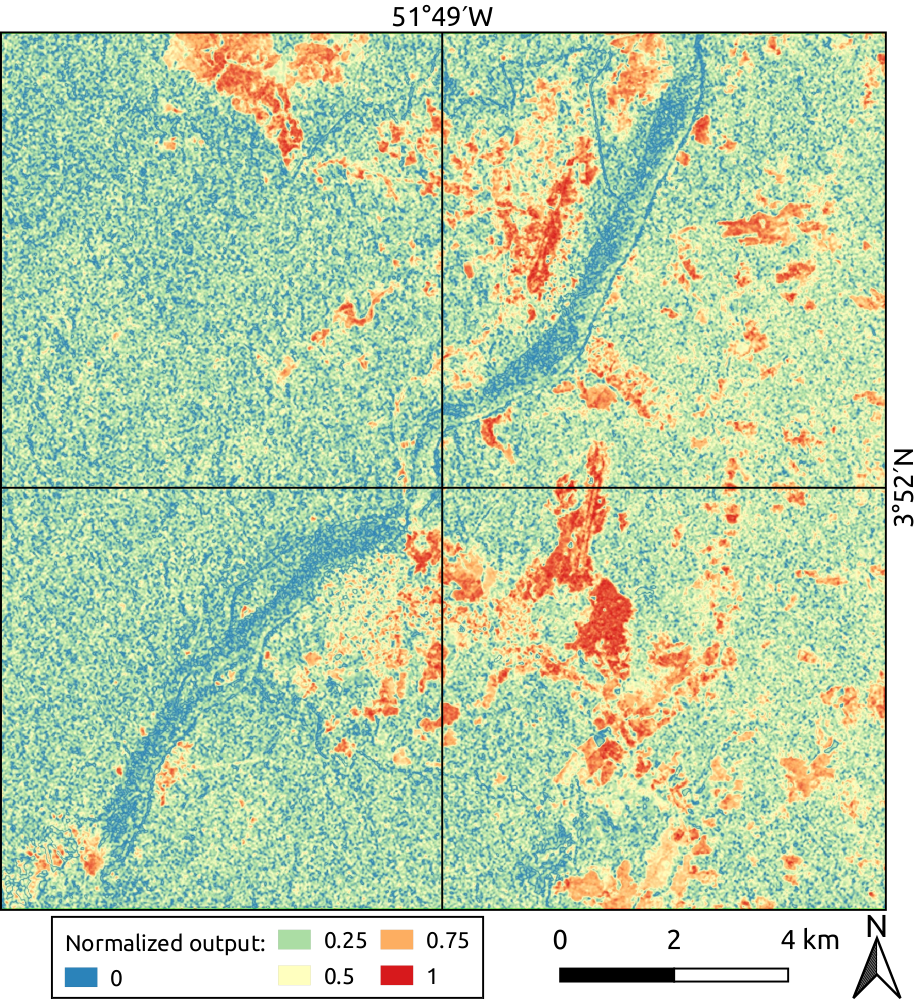
\includegraphics[width=0.23\textwidth]{../../qgis/maps/imageWECS.png}\label{imageWECS}} 
\subfigure[ECS -- $\widetilde{\vR}$]{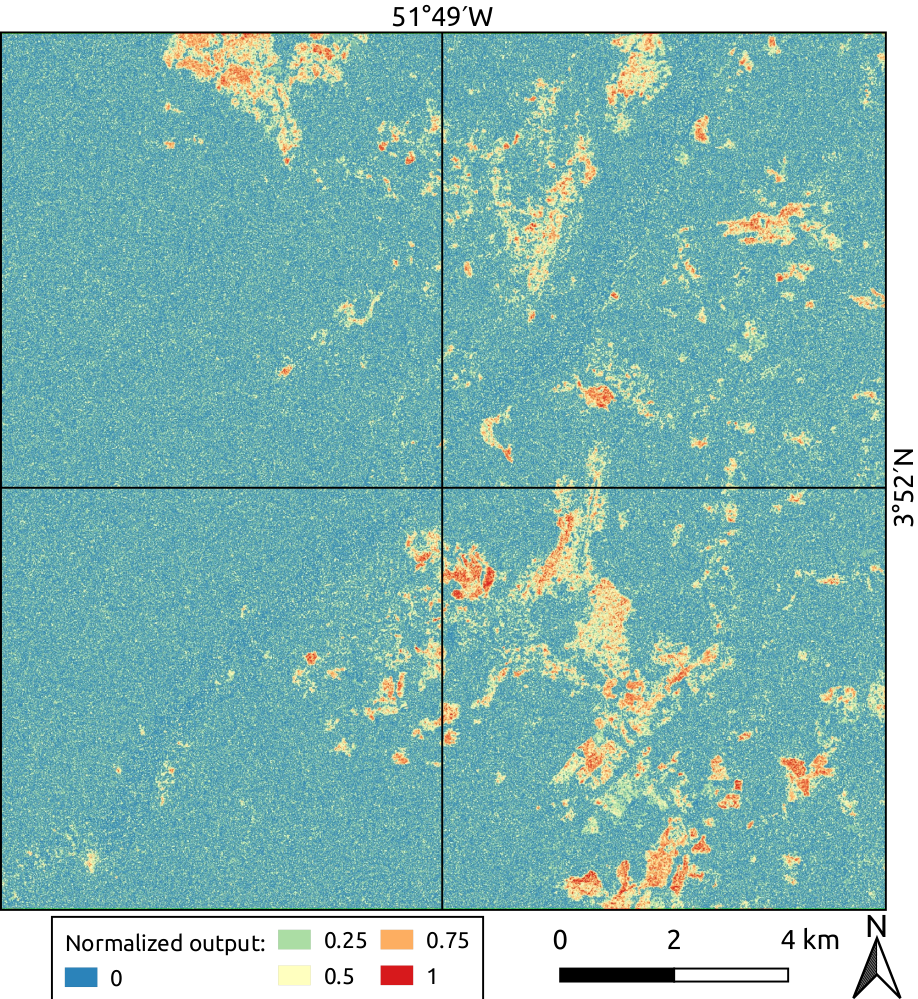
\includegraphics[width=0.23\textwidth]{../../qgis/maps/imageECS.png}\label{imageECS}}
}

\subfigure[TAAD -- $\vA$]{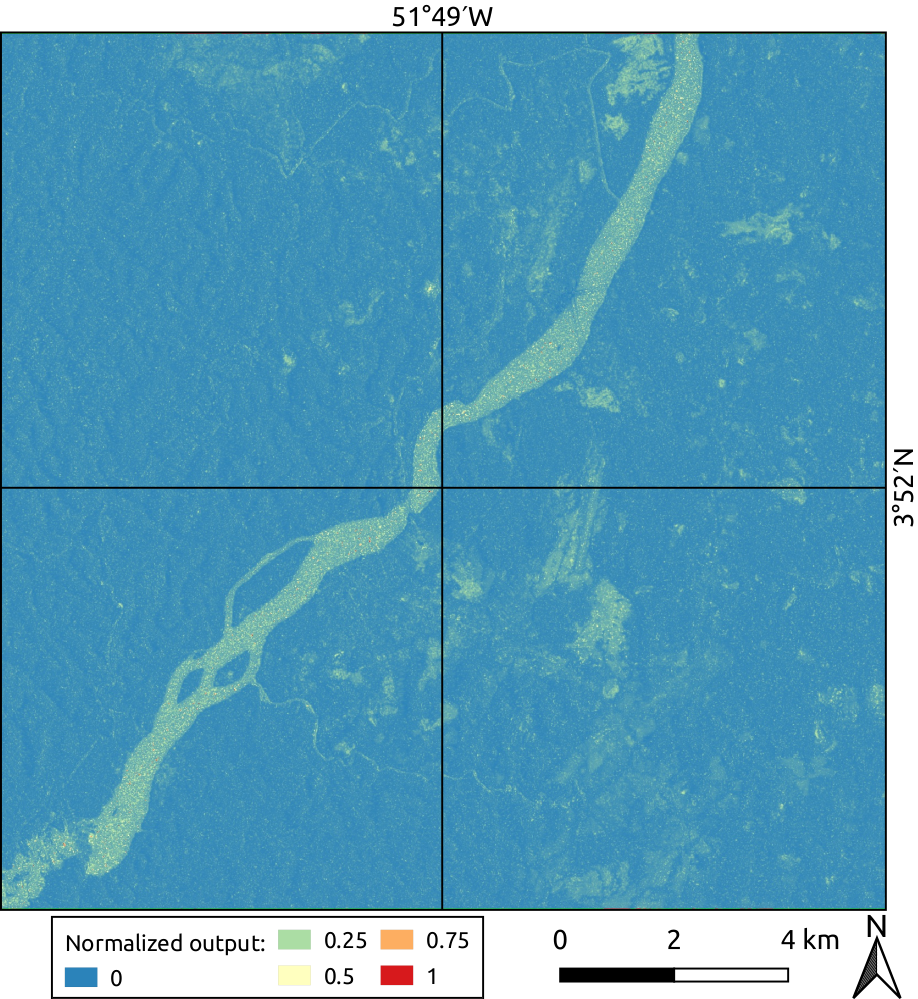
\includegraphics[width=0.23\textwidth]{../../qgis/maps/imageTAAD.png}\label{imageTAAD}}

\caption{The ``tendency of change'' matrices $\vR$, $\widetilde{\vR}$ and $\vA$  assigned to WECS, ECS and TAAD, respectively. The values are scaled to $[0,1]$.}\label{figImageMethods}
\end{figure}



%%%RGN: ler com calma o trecho abaixo...
According to the adopted accuracy measures, WECS, especially when submitted to the OT algorithm, presents a better performance detecting change locations without increasing/inflating the amount of false positives (FP), which is justified by a higher F1-Score level in comparison to the competitors ECS and TAAD. 
Moreover, according to the kappa coefficient, WECS also deliveries a more balanced correct classification regarding the change and non-change areas.
Furthermore, based on the kappa values and respective variances, it is verified that the difference between any pair of results is significant at 1\%.

Although WECS's performance when equipped with the KI algorithm is inferior to the OT algorithm, it is worth observing that the introduced methods still provide more accurate results than either ECS or TAAD.
Regarding the competitors, TAAD presents frequent FP errors, leading to lower F1-Score and kappa coefficient than ECS.



Figure~\ref{figSentinelResults} depicts the most accurate change/non-change maps according to the measures in Table~\ref{tabAccExpSentinel}.
It is possible to verify that, while TAAD-K1 assigns the water body as a ``region of change'', it does not detect locations that changed (northwest and southeast portions -- second and fourth quadrants).
Regarding ECS, its result has a noise-corrupt character, with frequent FP classification points.

As previously observed, WECS equipped with the KI algorithm provides a homogeneous mapping over the non-change areas (west portion -- second and third quadrants), accurate detection over the change regions, and low inclusion (FP) and exclusion (FN) error rates. In adopting the OT algorithm, the inclusion error increases, resulting in a less-regularized change/non-change map.

The proportions of True/False Positive/Negative assigned to the analyzed methods are shown in Figure~\ref{figTPTNs} and corroborate the aforementioned discussion.




\begin{table}[H]
\caption{Accuracy values summary. Variance of kappa multiplied by $\times 10^{5}$.}\label{tabAccExpSentinel}
\centering
\begin{tabular}{ccccccc}
\thickhline
 & \multicolumn{2}{c}{\textbf{WECS}} & \multicolumn{2}{c}{\textbf{ECS}} & \multicolumn{2}{c}{\textbf{TAAD}}\tabularnewline
Threshold & OT & KI & OT & KI & OT & KI\tabularnewline
\hline 
F1-Score & 0.940 & 0.876 & 0.6189 & 0.661 & 0.798 & 0.778\tabularnewline
Kappa & 0.818 & 0.698 & 0.535 & 0.513 & 0.244 & 0.284\tabularnewline
Var. of kappa & 6.90 & 3.43 & 1.91 & 1.72 & 0.76 & 0.91 \tabularnewline
\thickhline
\end{tabular}
\end{table}



%-----------------------
\begin{figure}[h!]
\centering

\mbox{
\subfigure[WECS-KI]{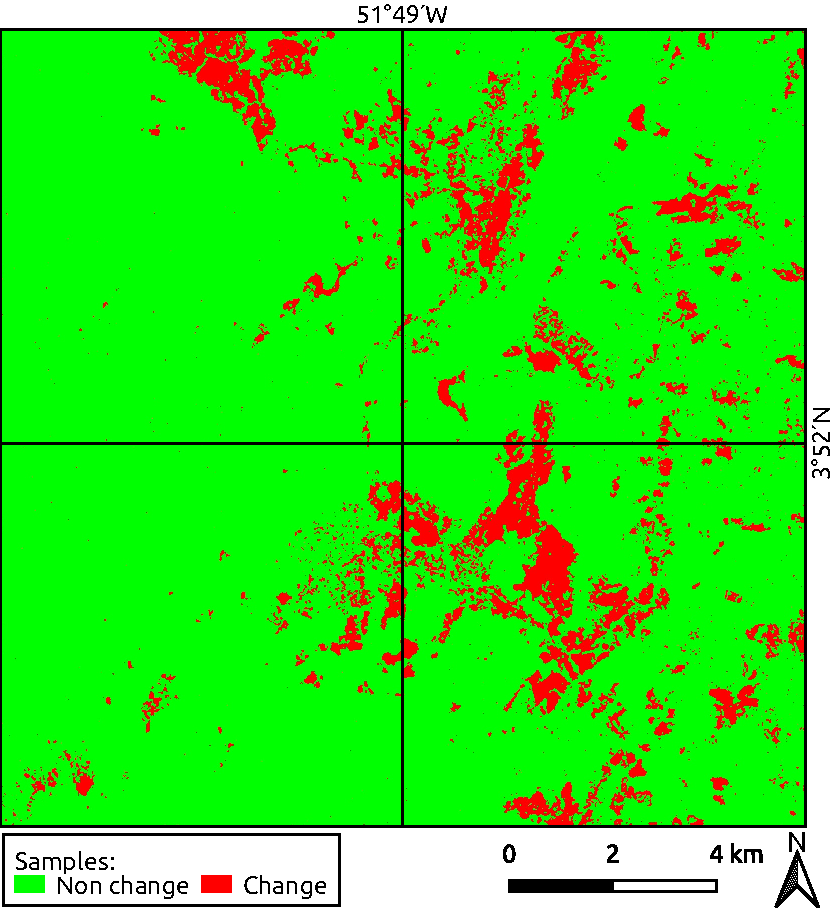
\includegraphics[width=0.23\textwidth]{../../qgis/maps/WECS-KI.pdf}\label{figResChange1}} 
\subfigure[WECS-OT]{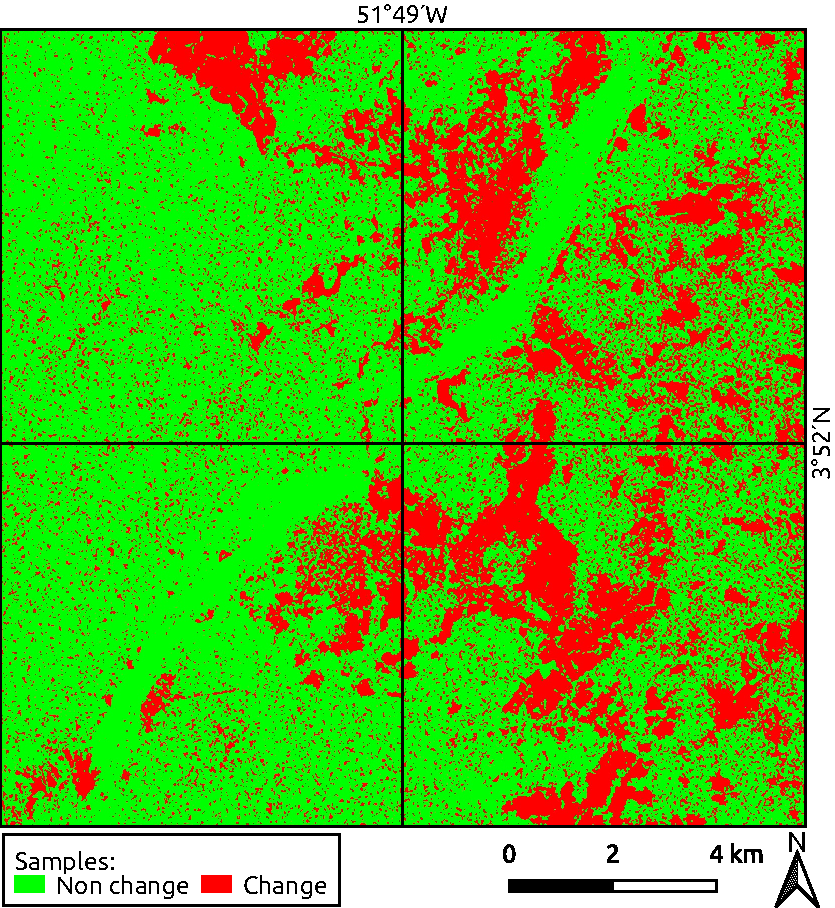
\includegraphics[width=0.23\textwidth]{../../qgis/maps/WECS-OT.pdf}\label{figResChange2}}
}

\mbox{
\subfigure[ECS-OT]{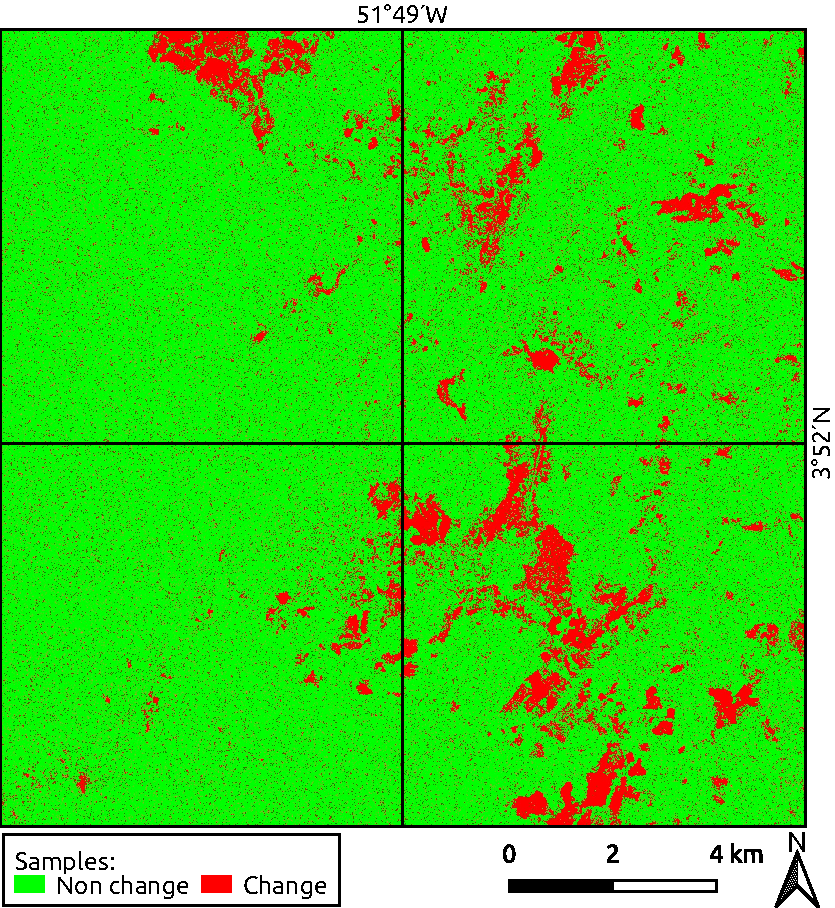
\includegraphics[width=0.23\textwidth]{../../qgis/maps/ECS-OT.pdf}\label{figResChange3}} 
\subfigure[TAAD-KI]{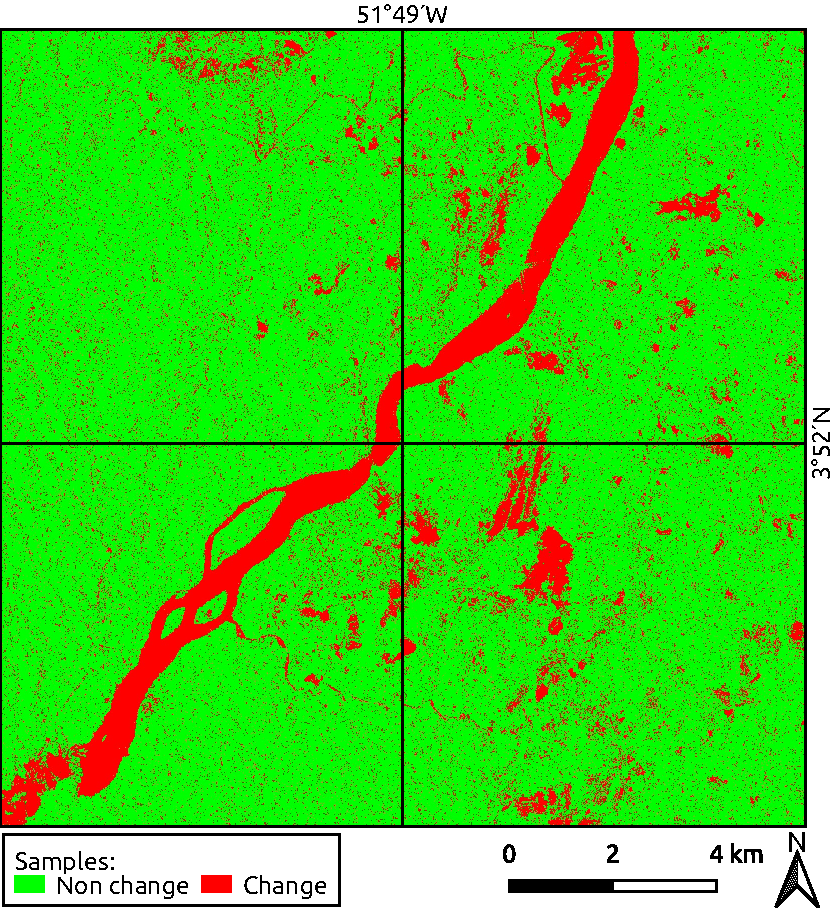
\includegraphics[width=0.23\textwidth]{../../qgis/maps/TAAD-KI.pdf}\label{figResChange4}}
}

\caption{Resulting change maps from the analyzed methods.}\label{figSentinelResults}
\end{figure}




%-----------------------
\begin{figure}[hbt]
\centering
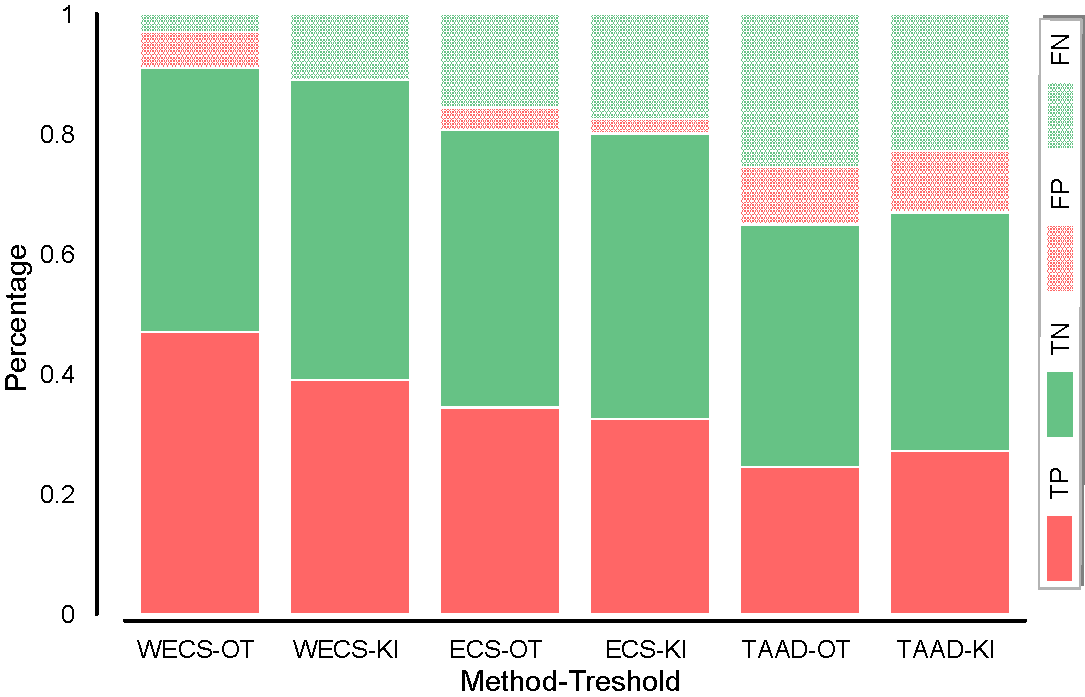
\includegraphics[width=0.485\textwidth]{../../graphs/TPTNs.pdf}
\caption{Percentages of True/False Positives (TP/FP) and True/False Negatives (TN/FN) relative to change (Positive) and non-change (Negative) reference samples.}\label{figTPTNs}
\end{figure}


Lastly, the computational run-time of WECS, TAAD and ECS were, respectively, \SI{143.45}{\second}, \SI{7.89}{\second} and \SI{110.08}{\second}. Despite expending a longer execution time, it is worth mention that WECS' running time is not excessive in the context of remote sensing image processing, beyond providing systematically more accurate results.




%%%%%%%%%%%%%%%%%%%%%%%%%%%%%%%%%%%%%%%%%%
\section{Conclusion}\label{section_discussion}


We present a novel way of detecting changes in multi-temporal satellite images called WECS. The procedure is based on wavelet energies from both the estimated individual coefficients as well as the whole mean image. It makes use of correlation screening for ultra-high dimensional data to identify which locations (pixels) are the most related to an overall change measure of the image time series. Thereupon, WECS is expected to provide a sample of points in space in a way that such set contains real change points with high probability. 

The performance of WECS was evaluated in studies involving simulated and real data. In both experiments, WECS is compared with two standard approaches for analyzing multi-temporal images. One drawback of WECS compared to standard methods is that it takes longer time to process the images. However, its performance is shown to be superior on both real and simulated image, and the processing time is still not prohibitive.

The current paper warrants future research in different directions, for example: adapting the idea of WECS to different types of images (multispectral, polarimetric SAR, etc); extending energy correlation screening for distinct smoothing techniques; deducing sharp theoretical change detection rates for appropriate statistical models.




% if have a single appendix:
%\appendix[Proof of the Zonklar Equations]
% or
%\appendix  % for no appendix heading
% do not use \section anymore after \appendix, only \section*
% is possibly needed

% use appendices with more than one appendix
% then use \section to start each appendix
% you must declare a \section before using any
% \subsection or using \label (\appendices by itself
% starts a section numbered zero.)
%

%
%\appendices
%\section{Proof of the First Zonklar Equation}
%Appendix one text goes here.

% you can choose not to have a title for an appendix
% if you want by leaving the argument blank
%\section{}
%Appendix two text goes here.


% use section* for acknowledgment
\section*{Acknowledgment}

The authors would like to thank the European Space Agency (ESA) for providing the Sentinel-1 data used in this research.


% Can use something like this to put references on a page
% by themselves when using endfloat and the captionsoff option.
\ifCLASSOPTIONcaptionsoff
  \newpage
\fi



% trigger a \newpage just before the given reference
% number - used to balance the columns on the last page
% adjust value as needed - may need to be readjusted if
% the document is modified later
%\IEEEtriggeratref{8}
% The "triggered" command can be changed if desired:
%\IEEEtriggercmd{\enlargethispage{-5in}}

% references section

% can use a bibliography generated by BibTeX as a .bbl file
% BibTeX documentation can be easily obtained at:
% http://mirror.ctan.org/biblio/bibtex/contrib/doc/
% The IEEEtran BibTeX style support page is at:
% http://www.michaelshell.org/tex/ieeetran/bibtex/
\bibliographystyle{IEEEtran}
% argument is your BibTeX string definitions and bibliography database(s)
\bibliography{bibfile}
%
%% <OR> manually copy in the resultant .bbl file
%% set second argument of \begin to the number of references
%% (used to reserve space for the reference number labels box)
%\begin{thebibliography}{1}
%
%\bibitem{IEEEhowto:kopka}
%H.~Kopka and P.~W. Daly, \emph{A Guide to \LaTeX}, 3rd~ed.\hskip 1em plus
%  0.5em minus 0.4em\relax Harlow, England: Addison-Wesley, 1999.
%
%\end{thebibliography}

% biography section
% 
% If you have an EPS/PDF photo (graphicx package needed) extra braces are
% needed around the contents of the optional argument to biography to prevent
% the LaTeX parser from getting confused when it sees the complicated
% \includegraphics command within an optional argument. (You could create
% your own custom macro containing the \includegraphics command to make things
% simpler here.)
%\begin{IEEEbiography}[{\includegraphics[width=1in,height=1.25in,clip,keepaspectratio]{mshell}}]{Michael Shell}
% or if you just want to reserve a space for a photo:


%\begin{IEEEbiography}
%[{\includegraphics[width=1in,height=1.25in,clip,keepaspectratio]{../Photo/rodney}}]{Rodney Fonseca}
%was born in Brazil, in 1993. He received the Master’s
%degrees in Statistics from the Federal University of Pernambuco,
%Recife, Brazil, in 2017, and the Ph.D. degree in Statistics, from Campinas State University, Campinas, Brazil, in 2021.
%His research interests include nonparametric statistics, time series, graph signal processing and regression models.
%\end{IEEEbiography}
%\vfill
%
%\begin{IEEEbiography}[{\includegraphics[width=1in,height=1.25in,clip,keepaspectratio]{../Photo/aluisio}}]{Alu\'{i}sio~Pinheiro}
%was born in Brazil, in 1967. He received the Master’s degree in Statistics from Campinas State University, Campinas, Brazil, in 1992, and the Ph.D. degree in Statistics from University of North Carolina, Chapel Hill, US, in 1997.
%He is currently Professor at Campinas State University. His research interests concern U-statistics, wavelets, nonparametric statistics and time series.
%Dr. Pinheiro was the 2012 Pranab Kumar Sen Distinguished Visiting Professor of Biostatistics, UNC-Chapel Hill. He has been the Brazilian Statistics Association General Secretary (2010-2012) and Treasurer (2018-2020).
%\end{IEEEbiography}
%
%
%\begin{IEEEbiography}[{\includegraphics[width=1in,height=1.25in,clip,keepaspectratio]{../Photo/abdou}}]{Abdourrahmane Mahamane Atto}
%was born in Niger, in 1974. He received the Master’s
%degrees in applied mathematics and pure mathematics from the University of Abomey-Calavi,
%Cotonou, Benin, 2001 and 2002, respectively, the
%Master’s degree of advanced studies in electrical engineering from the École Polytechnique d’Abomey-Calavi, Cotonou, in 2002, and the Ph.D. degree
%in applied mathematics, codelivered by TELECOM
%Bretagne, Brest, France, and the University of
%Rennes I, Rennes, France, in 2008.
%He worked with École Polytechnique d’Abomey-Calavi, from 2002 to 2003,
%Ecole des Mines, de l’Industrie et de la Géologie, Niamey, Niger, from 2003
%to 2004, TELECOM Bretagne, from 2008 to 2009, and Institut Polytechnique
%de Bordeaux, Talence, France, from 2009 to 2011. Since September 2011, he
%has been an Associate Professor at the University of Savoie, Polytech Annecy-Chambéry, Annecy, France. His research interests concern mathematical methods and models for signal, image, and information processing.
%\end{IEEEbiography}
%\vfill

% You can push biographies down or up by placing
% a \vfill before or after them. The appropriate
% use of \vfill depends on what kind of text is
% on the last page and whether or not the columns
% are being equalized.

%\vfill

% Can be used to pull up biographies so that the bottom of the last one
% is flush with the other column.
%\enlargethispage{-5in}



% that's all folks
\end{document}


